\documentclass[presentation]{beamer}
\usepackage{common}
\usepackage{arydshln}

\newcommand{\cscat}[1]{$\langle\text{{\itshape#1}}\rangle$}
\newcommand{\csopt}[1]{{\itshape[#1]}}
\newcommand{\csalt}[1]{{\itshape(#1)}}
\newcommand{\op}[1]{\alert{`\texttt{#1}'}}
\newcommand{\operand}[1][\ldots]{{\normalcolor#1}}
\newcommand{\literal}[1]{\texttt{\alert{#1}}}
\newcommand{\bs}{$\backslash$}
\newcommand{\codepath}[1]{../../code/lecture-02/#1}

\AtBeginSubsection[]
{
  \begin{frame}<beamer>
    \frametitle{Next In Line\ldots}
    \tableofcontents[currentsection,currentsubsection]
  \end{frame}
}

\title[\lecturecode{02}]{02 \\ \dotnet and \csharp Fundamentals}

\author[Giovanni Ciatto]{Giovanni Ciatto\\\texttt{giovanni.ciatto@unibo.it}}

\begin{document}

\frame[label=coverpage]{\titlepage}

\section{\dotnet Overview}

\begin{frame}{What is \dotnet}
    \begin{block}{Definition}\centering
        \dotnet is a free, general-purpose, open-source, and multi-platform \emph{programming ecosystem}
    \end{block}  

    \vfill

    \begin{description}
        \item[programming ecosystem] | as it comprehends several languages, compilers, tools, libraries, etc.
        
        \vfill

        \item[multi-platform] | as it can be used on several OS and architectures (e.g. Win, Linux, MacOs, Android, etc)
        
        \vfill

        \item[open-source] | as its source code is publicly available and openly licensed
        
        \vfill

        \item[general-purpose] | as it supports several sorts of applications (e.g. desktop, mobile, web, videogames, databases, etc)
        
        \vfill

        \item[free] | as it is can be exploited with no additional costs
    \end{description}
\end{frame}

\begin{frame}[allowframebreaks]{\dotnet in a Nutshell}
    \begin{center}
        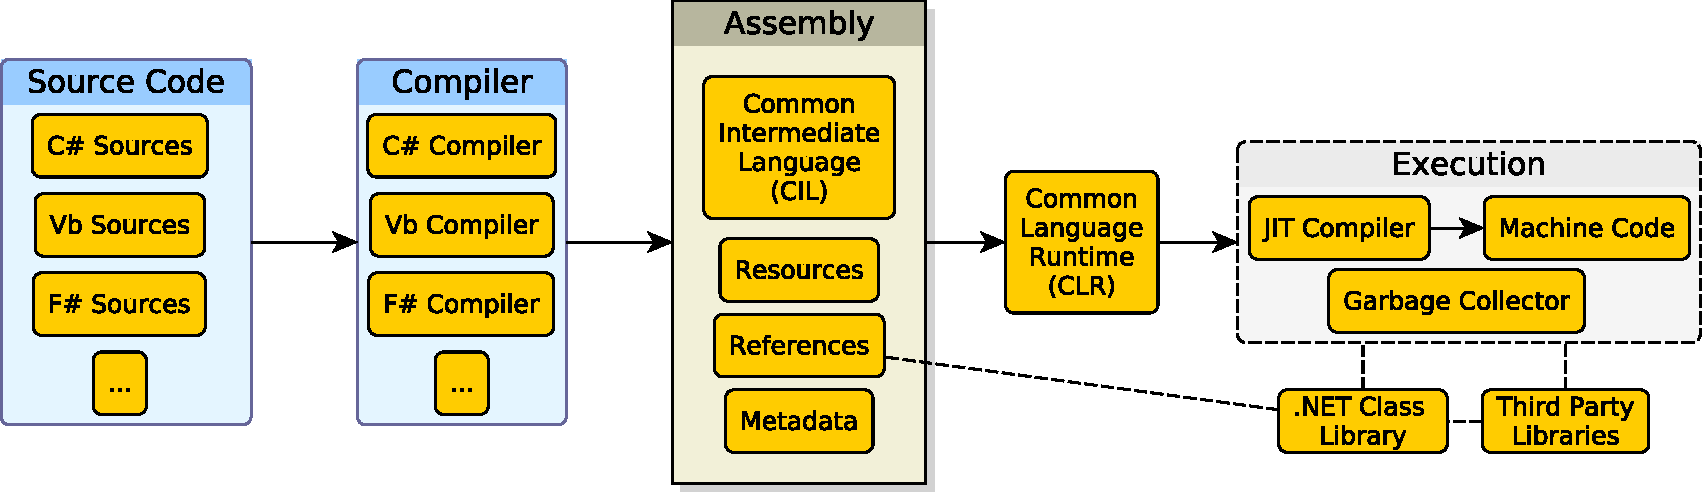
\includegraphics[width=\linewidth]{img/dotnet-overview.pdf}
    \end{center}

    \framebreak

    \begin{enumerate}
        \item Sources written using disparate \alert{languages} (e.g. \csharp, Vb, F\#, etc.)
        
        \smallskip

        \item can be compiled, via as many \alert{compilers}
        
        \smallskip

        \item into \alert{assemblies} containing
        %
        \begin{description}
            \item[common intermediate language (CIL)] |  a language- and platform-agnostic, compiled version of the sources
            \item[references] | dependencies declarations for the assembly
            \item[resources] | non-code files (e.g. internationalization strings, icons, default configurations, etc.) 
            \item[metadata] | for identifying the specific \emph{version} of the assembly
        \end{description}

        \smallskip
        
        \item which can then be executed by the \alert{common language runtime} (CLR) 
        %
        \begin{itemize}
            \item essentially, an \emph{interpreter} for the CIL
        \end{itemize}

        \smallskip

        \item  on any platform, via a \alert{just in time} (JIT) conversion into \alert{machine code}.
        
        \framebreak

        \item Execution of \dotnet code is \emph{managed} by default, meaning that:
        %
        \begin{itemize}
            \item developers must not take care of allocating/freeing memory
            \item as a \alert{garbage collector} is in charge of dynamically taking care of that
        \end{itemize}

        \bigskip

        \item \dotnet programs may reference (a.k.a. depend upon) other assemblies, such as
        %
        \begin{itemize}
            \item the \alert{\dotnet class library}, containing the standard SDK
            \item \alert{third party libraries}, either locally or remotely available
        \end{itemize}
        %
        and therefore exploit any class therein contained.

    \end{enumerate}
\end{frame}

\begin{frame}{\dotnet Platform -- The Present}
    \begin{center}
        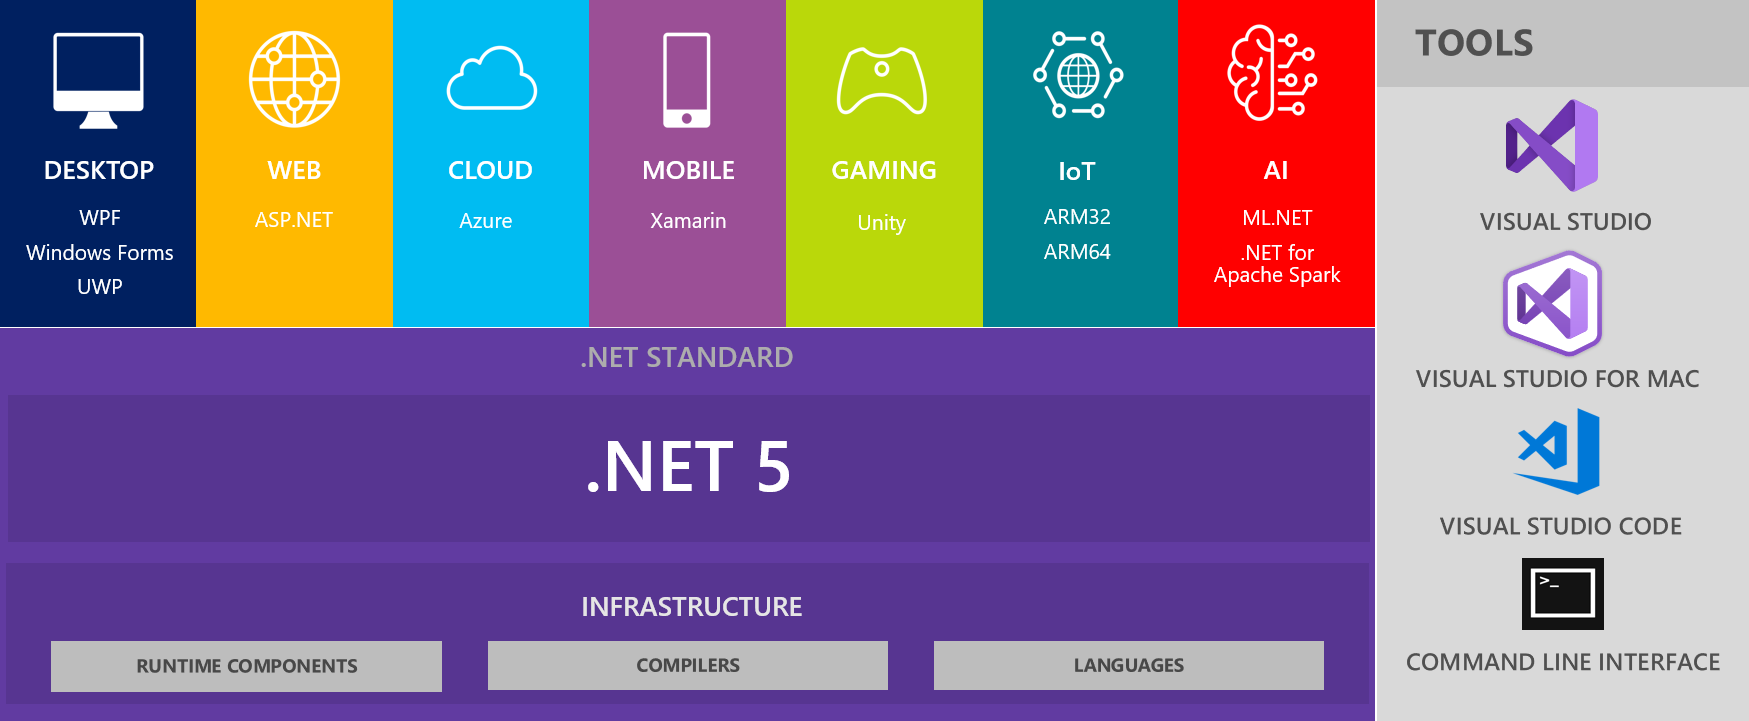
\includegraphics[width=\linewidth]{img/dotnet-overview-present.png}
    \end{center}
\end{frame}

\begin{frame}{\dotnet Platform -- The Past}
    \begin{center}
        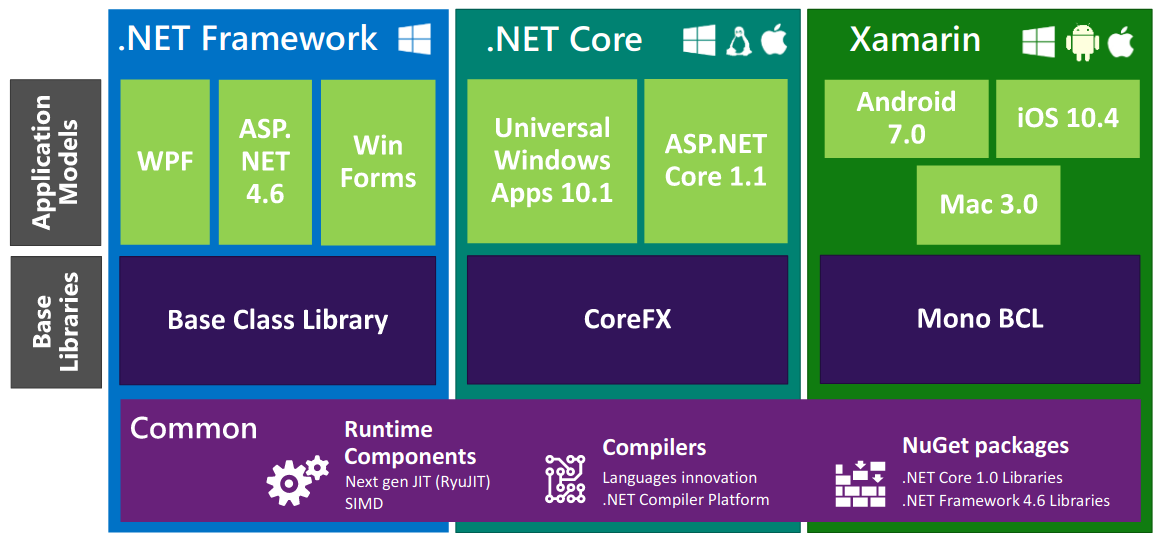
\includegraphics[width=\linewidth]{img/dotnet-overview-past.png}
    \end{center}
\end{frame}

\begin{frame}{\dotnet Platform -- Present vs. Past}
    \begin{itemize}
        \item Before \dotnet 5 there used to be three major implementations of the \emph{class library}:
        %
        \begin{description}
            \item[\dotnet Framework] | Windows-specific, full-featured, targetting desktop and web applications
            \item[\dotnet Core] | multi-platform (Win, Mac, Linux), less-featured, targetting desktop and web applications
            \item[Xamarin] | mobile-oriented (Android, iOS, Mac OS) 
        \end{description}

        \vfill

        \item Since \dotnet 5, implementations are aligned
    \end{itemize}

    \vfill

    \begin{alertblock}{In this course}\centering
        We stick to \alert{\dotnet Core 3.1}, to maximise interoperability and to avoid compatibility issues
    \end{alertblock}
\end{frame}

\section{Code Base Organization}

\subsection{Overview}

\begin{frame}[allowframebreaks]{Overview about Code Base Organization}
    \begin{center}
        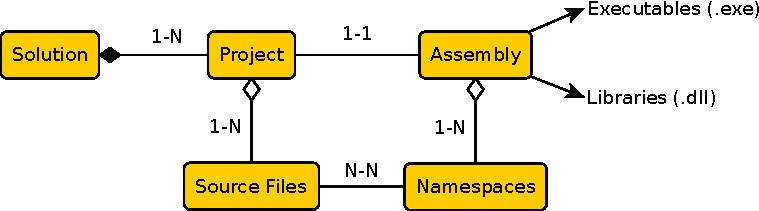
\includegraphics[width=\linewidth]{img/code-base.pdf}
    \end{center}

    \medskip

    \begin{enumerate}
        \item A \dotnet code base is called \alert{solution}
        
        \bigskip

        \item Each solution is a set of one or more related \alert{projects}
        %
        \begin{itemize}
            \item each project can contain sources written using a single \dotnet language
            \item different projects may target different \dotnet languages
            \item each project esplicitly targets one \emph{application model}
            %
            \begin{itemize}
                \item[eg] Class Library, Console/WinForms/WPF/Web Application, etc.
            \end{itemize}
        \end{itemize}

        \framebreak

        \item Each project is compiled into an \alert{assembly}
        %
        \begin{itemize}
            \item assemblies can either be executable or not---i.e. they can be \emph{libraries}
            \item executable assemblies have the \texttt{.exe} extension 
            \item library assemblies have the \texttt{.dll} extension
        \end{itemize}

        \medskip

        \item Each project is a container of several \alert{source} files 
        %
        \begin{itemize}
            \item containing several classes, structures, interfaces, or delegates definitions
            \item possibly organised into a number of \alert{namespaces}
        \end{itemize}

        \medskip

        \item Therefore, each assembly may \emph{expose} a number of namespaces, along with their definitions
    \end{enumerate}

    \bigskip

    \begin{block}{Takeway}\centering
        Assemblies (and therefore projects) are \emph{deployment} and \emph{execution} \alert{units}
    \end{block}
\end{frame}

\begin{frame}{Code Base Organization Enforcement}
    \begin{itemize}
        \item Tools (such as IDEs) \emph{enforce} such code base organization
        
        \bigskip

        \item You can expect all \dotnet-enabled tools to stick to this organization
        %
        \begin{itemize}
            \item[eg] Visual Studio (VS) or JetBrain Rider
        \end{itemize}

        \bigskip

        \item Analogies exists with other IDEs:
        \smallskip
        \begin{center}
            \begin{tabular}{c||c|c|c}
                & \textbf{VS/Rider} & \textbf{Eclipse} & \textbf{Idea} \\
                \hline\hline
                \textbf{Code Base}       & Solution          & Workspace        & Project       \\
                \hline
                \textbf{Deployment Unit} & Project           & Project          & Module       
            \end{tabular}
        \end{center}
    \end{itemize}
\end{frame}

\subsection{Directory Structure}

\begin{frame}[allowframebreaks]{Canonical Directory Structure of a \dotnet Solution}
    \begin{center}
        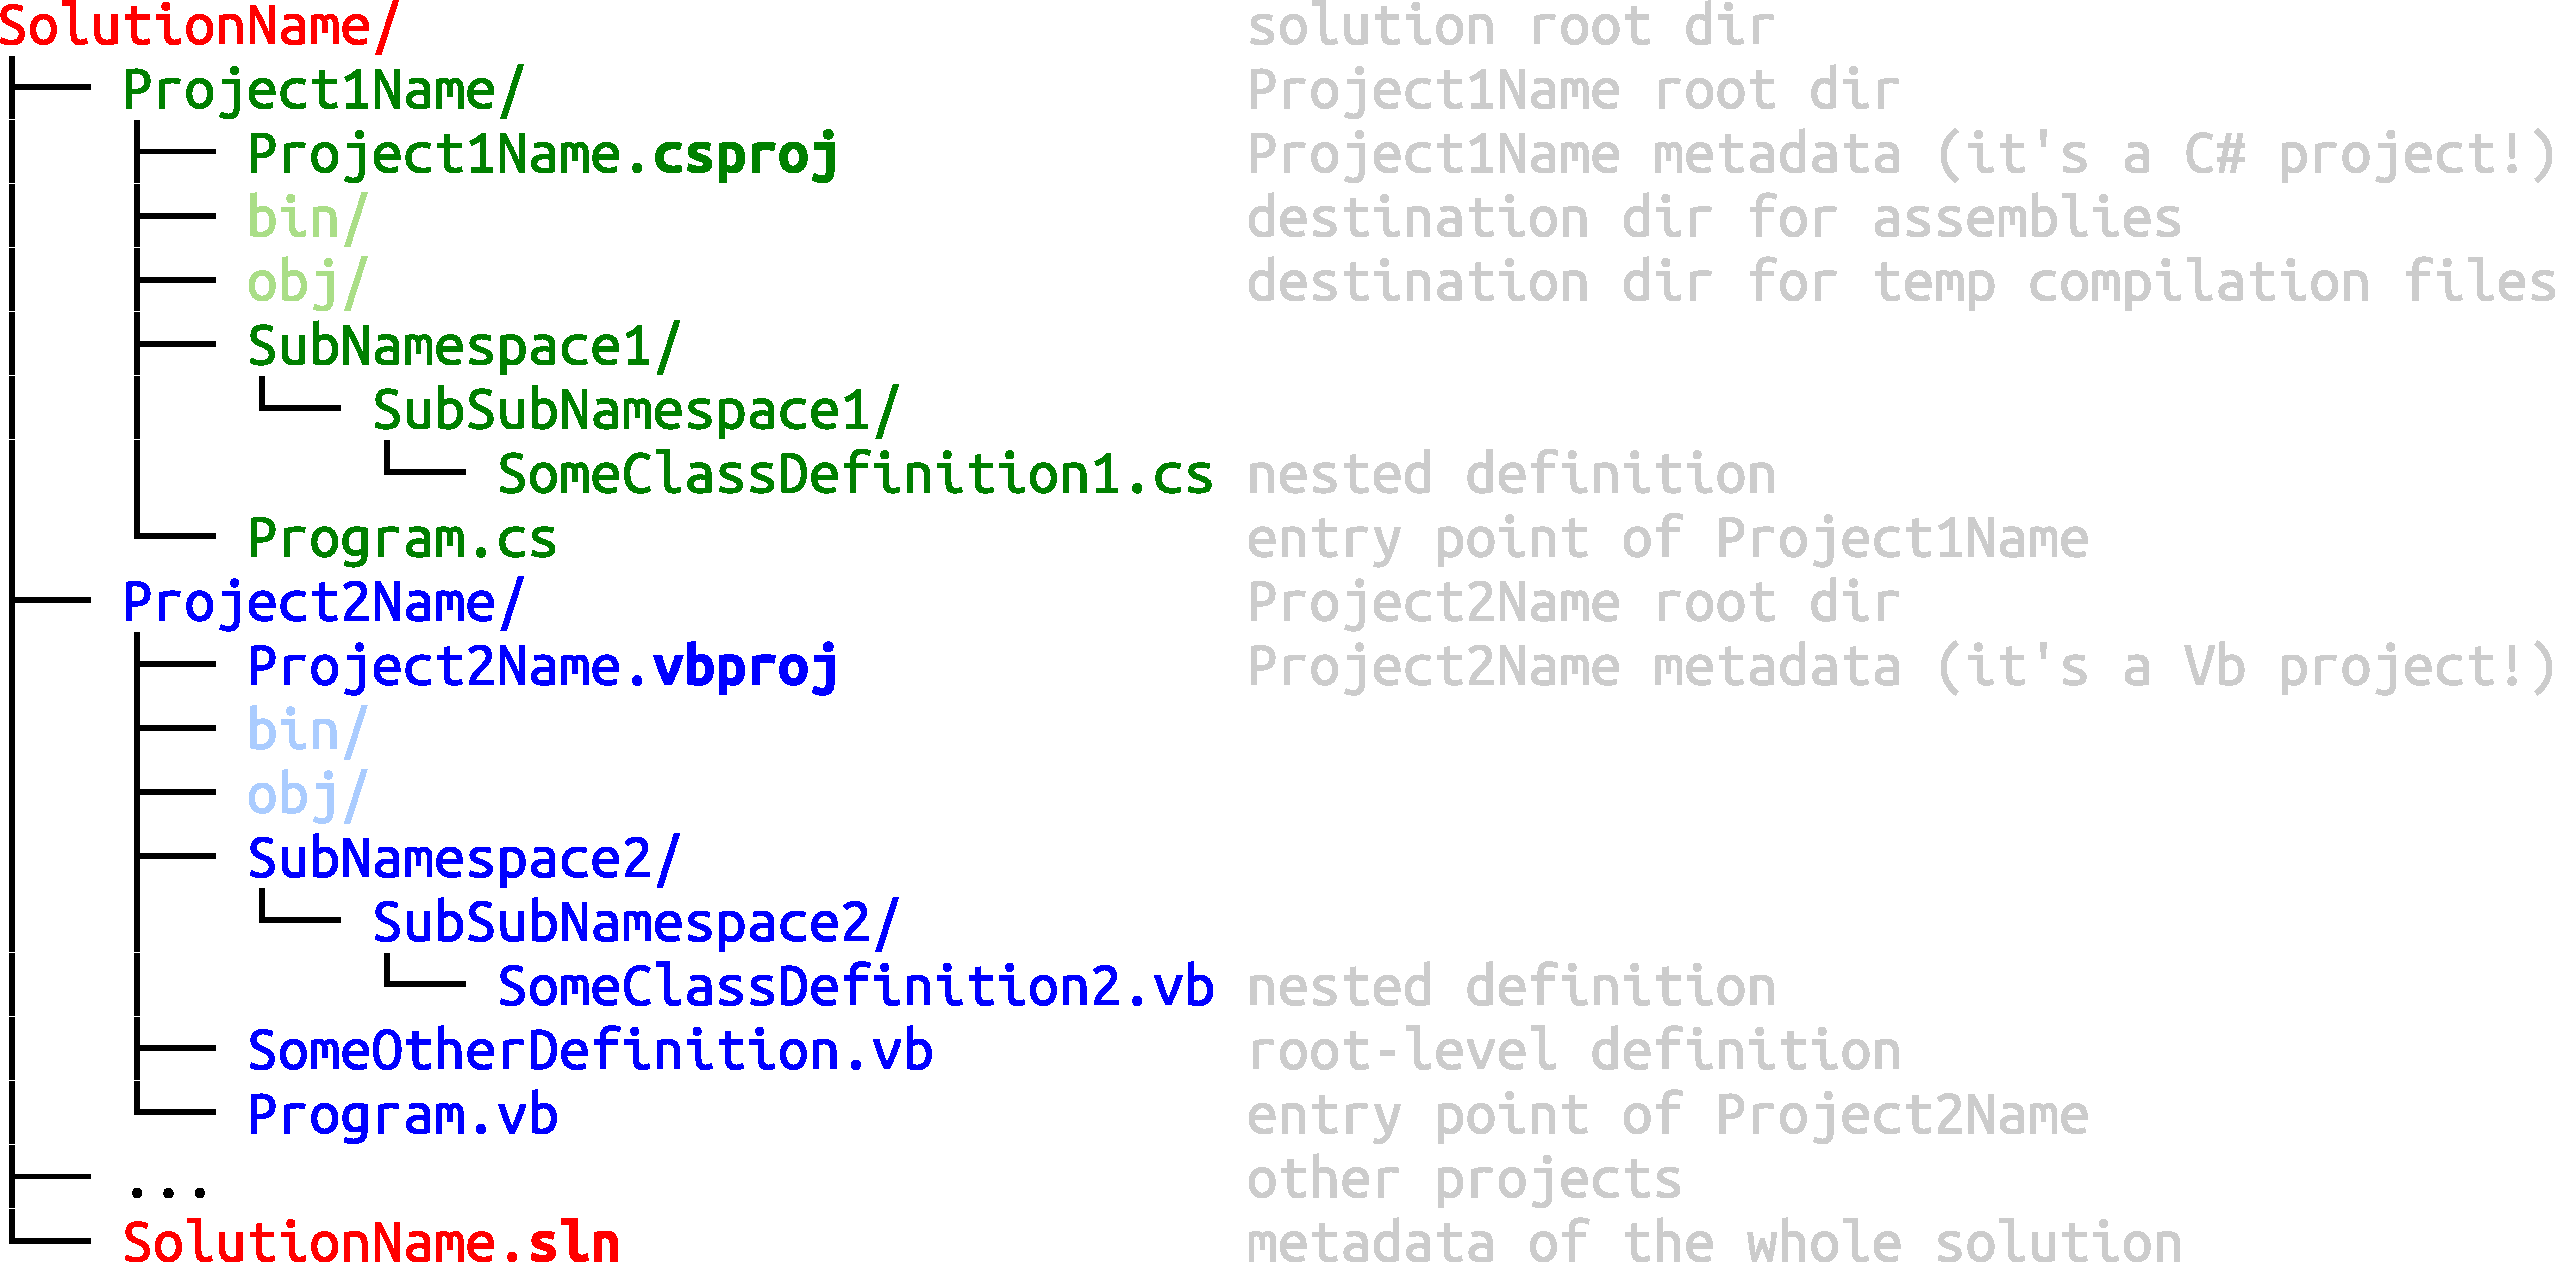
\includegraphics[width=\linewidth]{img/project-structure.pdf}
    \end{center}

    \framebreak

    \begin{itemize}
        \item Each solution $S$ has its own directory -- named $S$  -- containing:
        %
        \begin{itemize}
            \item a single \alert{$S$\texttt{.sln}} file
            \item a sub-directory for each project
        \end{itemize}

        \bigskip

        \item Each project $P$ has its own directory -- named $P$ --, within the solution directory, containing:
        %
        \begin{itemize}
            \item a single \alert{$P$\texttt{.csproj}} file (or $P$\texttt{.vbproj} for Vb projects)
            \item a directory for each namespace
            %
            \begin{itemize}
                \item possibly containing other sub-namespaces (and their directories)
                \item containing \texttt{.cs} source files (or \texttt{.vb} for Vb projects)
            \end{itemize}
            \item two directories, namely \texttt{bin/} and \texttt{obj/}, automatically generated
            \item some root-level \texttt{.cs} source files (or \texttt{.vb} for Vb projects)
        \end{itemize}

        \bigskip

        \item Conventionally, \emph{executable} projects contain a root-level \texttt{Program.cs} (or \texttt{.vb}) file
        %
        \begin{itemize}
            \item containing a \texttt{Main} method which is the \alert{entry proint} of the program
        \end{itemize}
    \end{itemize}
\end{frame}

\begin{frame}[allowframebreaks]{Example of \texttt{.sln} File}

    \lstinputlisting[basicstyle=\tiny\ttfamily]{\codepath{lecture-02.sln}}
    %
    \begin{itemize}
        \item[!] This is not somithing a developer may manually write!
    \end{itemize}
\end{frame}

\begin{frame}{Example of \texttt{.csproj} File}

    \lstinputlisting[basicstyle=\tiny\ttfamily]{\codepath{GreetingCLI/GreetingCLI.csproj}}
    %
    \begin{itemize}
        \item[!] This is not something a developer may comfortably manipulate!
    \end{itemize}
\end{frame}

\subsection{Handling a Solution}

\begin{frame}[allowframebreaks]{Handling a Solution via the Command Line}

    \begin{block}{The \texttt{dotnet} tool}
        \begin{itemize}
            \item All modern \dotnet installations comprehend a command-line tool named \alert{\texttt{dotnet}}
            \item It is the simpler way to handle a solution \emph{without} an IDE
            \item Among the many functionalities, it allows developers to:
            %
            \begin{enumerate}
                \item create a solution
                \item add projects to a solution
                \item compile a project into an assembly
                \item execute an executable assembly
                \item etc.
            \end{enumerate} 
        \end{itemize}
    \end{block}

    \begin{block}{How to use the \texttt{dotnet} tool}
        \begin{itemize}
            \item General syntax (square brackets denote optionality):
            %
            \begin{center}\centering\ttfamily\footnotesize
                \alert{\$} dotnet [sdk-options] [command] [command-options] [arguments]
            \end{center}

            \item How to learn how to use \texttt{dotnet}:
            %
            \begin{itemize}
                \item Run \texttt{dotnet [command] --help}
                \item See \url{https://docs.microsoft.com/dotnet/core/tools/dotnet}
            \end{itemize}
        \end{itemize}
    \end{block}

    \begin{exampleblock}{How to create \& manage a a solution with via \texttt{dotnet}}
        \begin{enumerate}
            \item Create a directory for the solution, say \texttt{MySolution}
            \item Open a shell into that directory
            \item Create an empty \texttt{.sln} file named after the current directory (i.e. \texttt{MySolution}):
            %
            \begin{itemize}\ttfamily
                \item[\$] dotnet new sln
            \end{itemize}
            \item Create a \csharp console app. project named \texttt{MyConsoleProject}:
            %
            \begin{itemize}\ttfamily\footnotesize
                \item[\$] dotnet new console -n MyConsoleProject -o MyConsoleProject
                \normalfont 
                \item[] (where \texttt{-n} indicates the project name, and \texttt{-o} its relative path) 
            \end{itemize}
            \item Register \texttt{MyConsoleProject} into \texttt{MySolution.sln}:
            %
            \begin{itemize}\ttfamily\footnotesize
                \item[\$] dotnet sln add MyConsoleProject/MyConsoleProject.csproj
                \normalfont 
                \item[] (recall to use \texttt{`\bs{}'} instead of \texttt{`/'} on Windows systems) 
            \end{itemize}    
            \item Run \texttt{MyConsoleProject} (re-compilation is implicit):
            %
            \begin{itemize}\ttfamily
                \item[\$] dotnet run --project MyConsoleProject/MyConsoleProject.csproj
            \end{itemize}
        \end{enumerate}
    \end{exampleblock}
    
\end{frame}

\begin{frame}[allowframebreaks]{Handling a Solution via the IDE}

    \begin{block}{Disclaimer}
        \begin{itemize}
            \item Using the command line may be hard, but it is free
            \item IDEs (e.g. Rider or VS) may be used instead, but they require a license
            \item We provide instructions for Rider, as it is multi-platform
            \item Apart for the appearance, VS is functionally very similar to Rider
            %
            \begin{itemize}
                \item as they rely on the same abstractions (solution, project, assembly, etc.)
            \end{itemize}
        \end{itemize}
    \end{block}

    \framebreak

    \begin{enumerate}
        \item Open your IDE
        %
        \begin{center}
            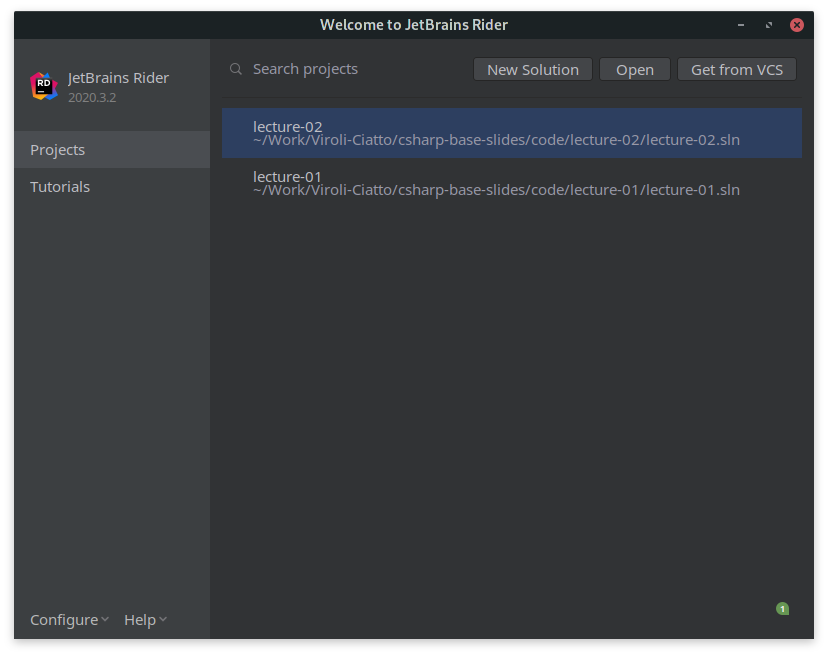
\includegraphics[width=.6\linewidth]{img/rider-1.png}
        \end{center}
        %
        (if you cannot see the welcome dialog above, then click on \alert{`File'} $\rightarrow$ \alert{`New\ldots'} to proceed)

        \framebreak

        \item Click on \alert{`New Solution'}
        %
        \begin{center}
            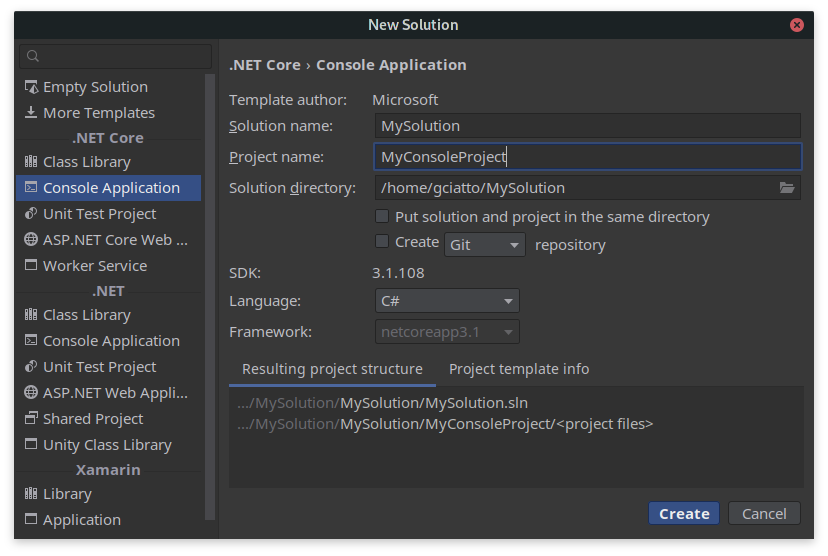
\includegraphics[width=.6\linewidth]{img/rider-2.png}
        \end{center}
        %
        \begin{enumerate}
            \item Choose the \emph{`Console Application'} template from the \emph{`\dotnet Core'} group
            \item Set the \emph{`Solution Name'} to \texttt{`MySolution'}
            \item Set the \emph{`Project Name'} to \texttt{`MyConsoleProject'}
            \item Ensure the \emph{`Solution Directory'} ends with \texttt{`MySolution'}
            \item Press the \alert{`Create'} button
        \end{enumerate}

        \framebreak

        \item The IDE should now appear like this:
        %
        \begin{center}
            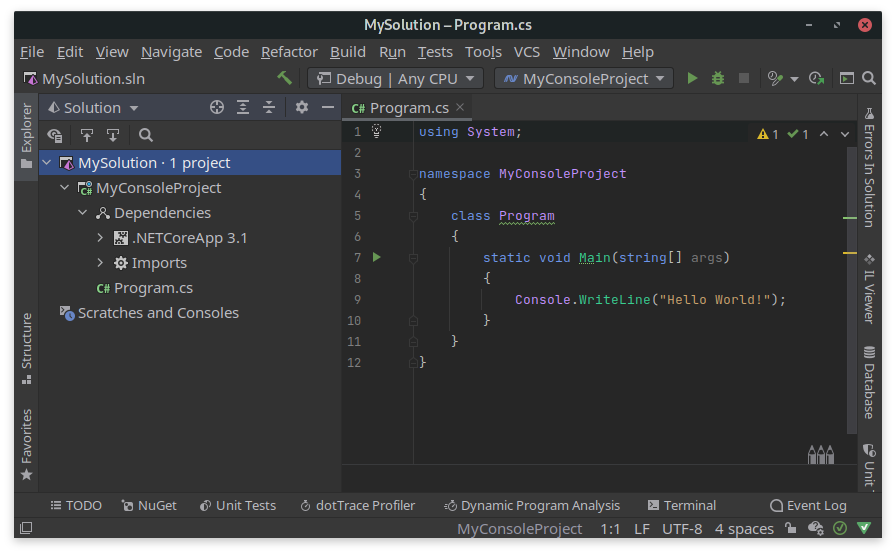
\includegraphics[width=.6\linewidth]{img/rider-3.png}
        \end{center}
        %
        \begin{itemize}
            \item The \emph{Solution Explorer} view (here on the left) shows all the projects, along with their source files, dependencies (a.k.a. references), and resource files
            \item You can use that to browse the code base or you can \alert{Ctrl+Click} any symbol of any source file to jump to its definition
        \end{itemize}

        \framebreak

        \item You may use the \alert{`Play'} or \alert{`Bug'} button to run a project
        %
        \begin{center}
            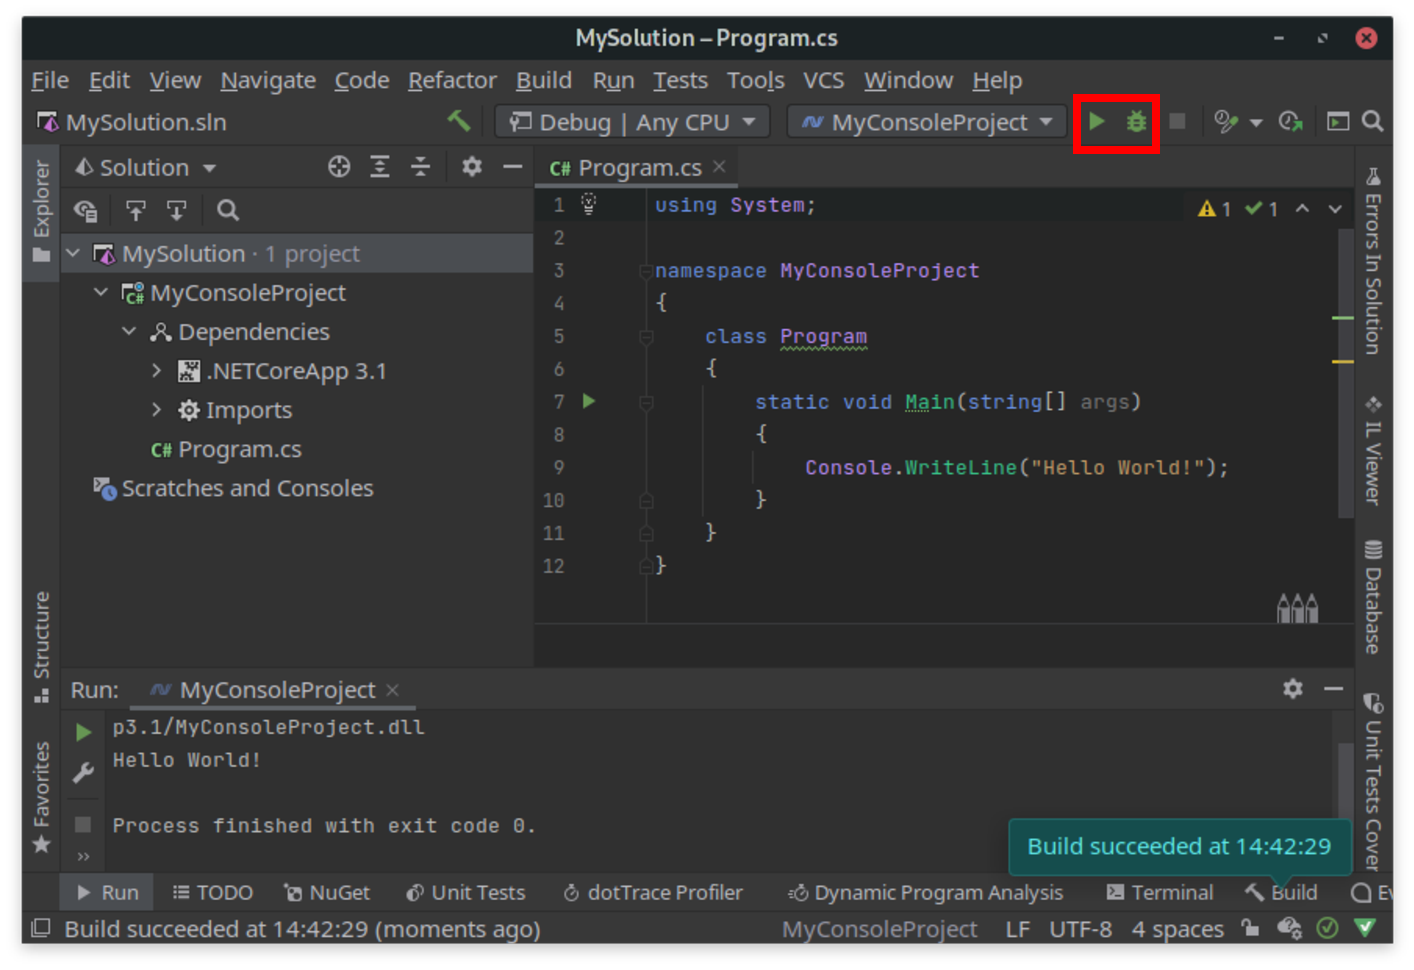
\includegraphics[width=.6\linewidth]{img/rider-4a}
        \end{center}
        %
        \begin{itemize}
            \item The output of the program appears either below (Rider) or into a new window (VS)
            \item The `Play' appears close to the \texttt{Main} method as well
        \end{itemize}

        \framebreak

        \item Which project is actually run when you press `Play' depends on which project is currently selected:
        %
        \begin{center}
            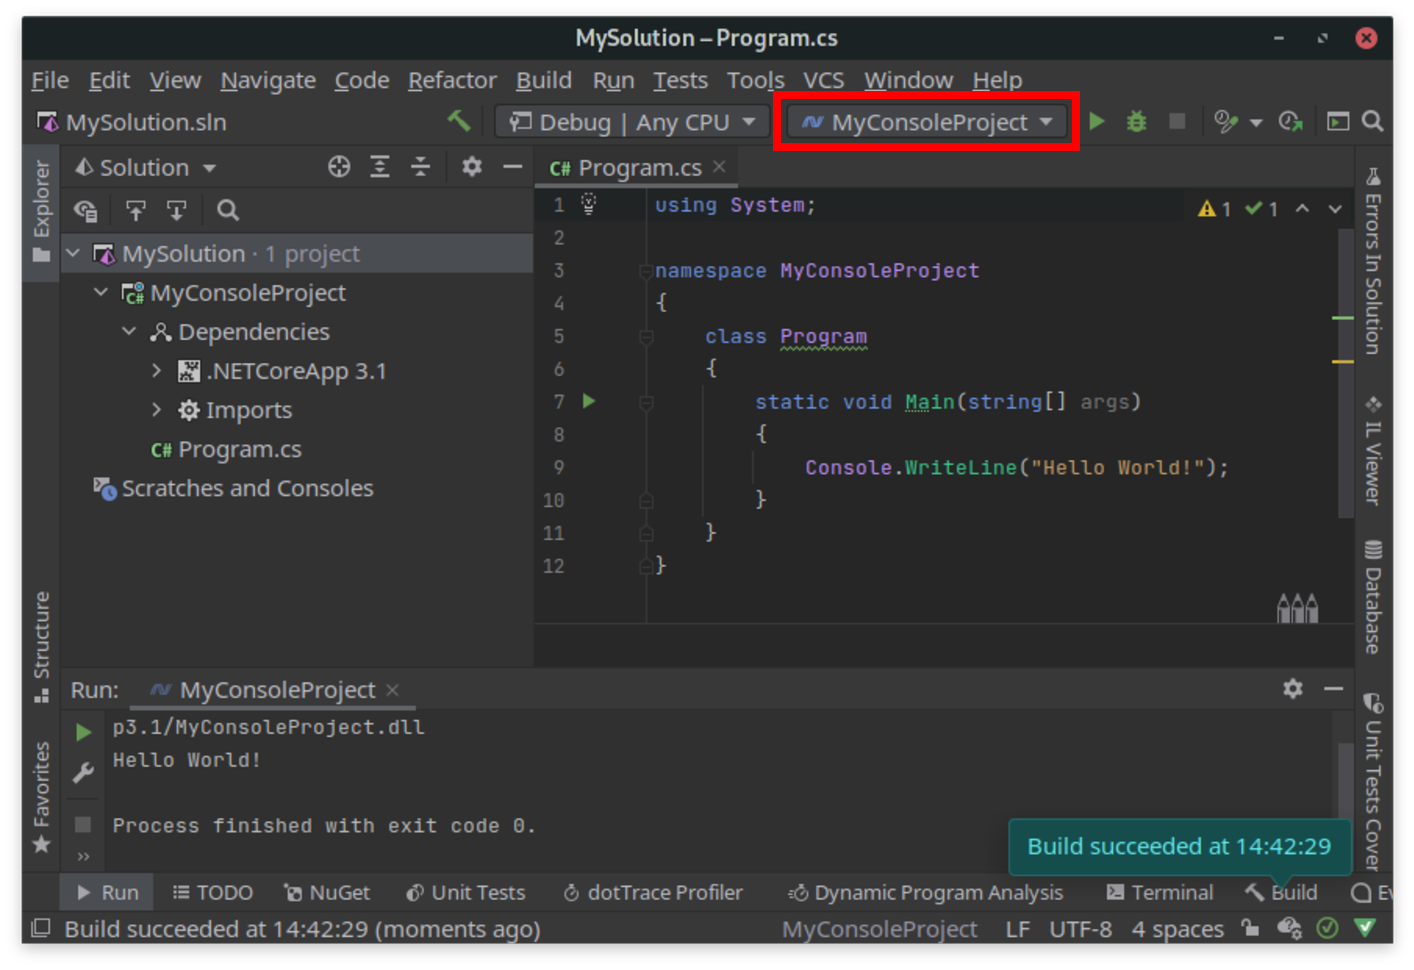
\includegraphics[width=.6\linewidth]{img/rider-4b}
        \end{center}
        %
        \begin{itemize}
            \item Only \emph{executable} projects can be selected on that menu
            \item Recall that each executable project has a single \emph{entry point}
            %
            \begin{itemize}
                \item[ie] its \alert{\texttt{static void Main}} method
            \end{itemize}
        \end{itemize}

        \framebreak

        \item Assemblies may be compiled either in \alert{`Debug'} or in \alert{`Release'} mode:
        %
        \begin{center}
            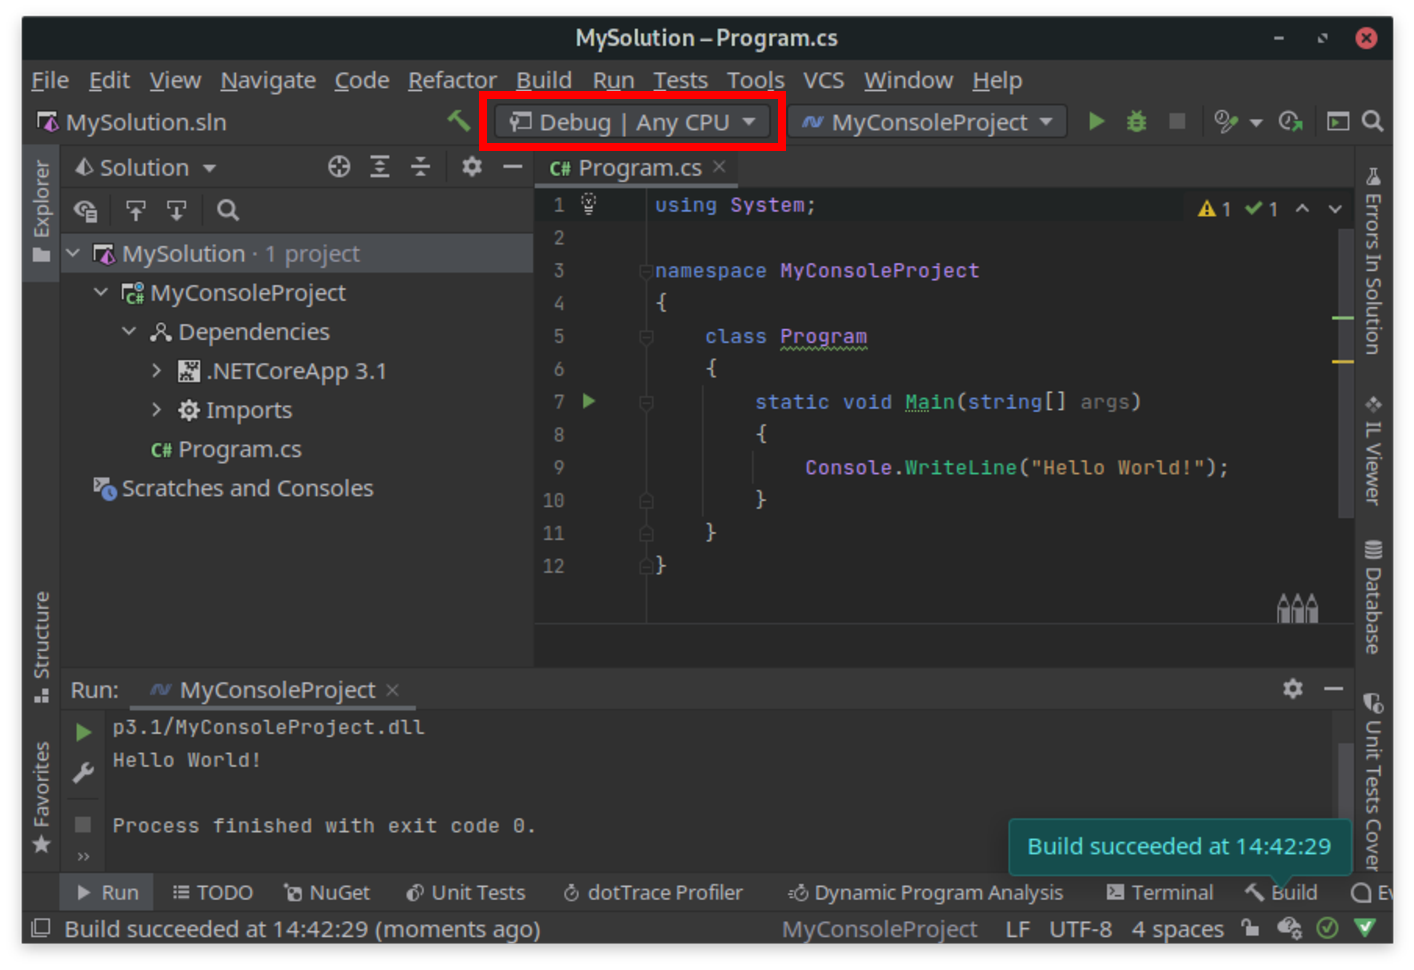
\includegraphics[width=.6\linewidth]{img/rider-4c}
        \end{center}
        %
        \begin{itemize}
            \item When compiled in `Release' mode, optimisation are performed, which makes step-by-step debugging hard as some instructions may be pruned
            \item When compiled in `Debug' mode, no optiomisation is performed
        \end{itemize}

        \framebreak

        \item You may click close to a code line to set up a \alert{breakpoint} on that line
        %
        \begin{center}
            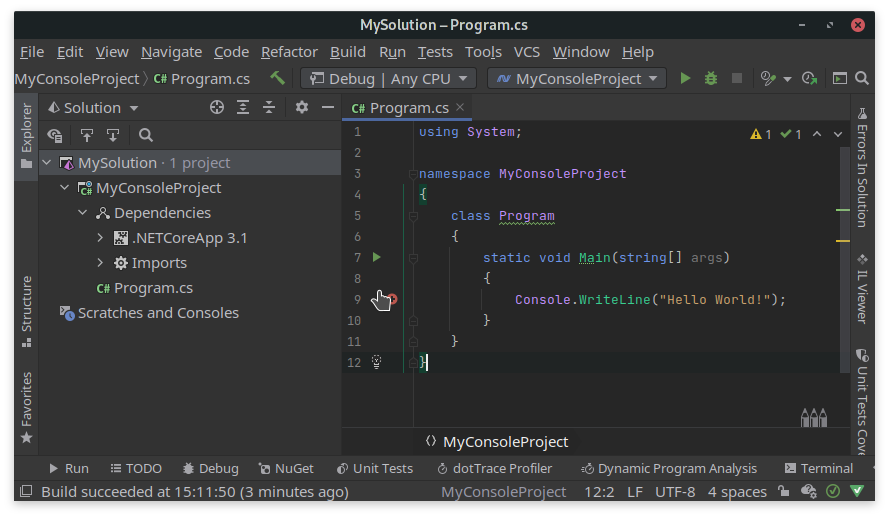
\includegraphics[width=.6\linewidth]{img/rider-5}
        \end{center}
        %
        \begin{itemize}
            \item breakpoints are \emph{ignored} when launching the program with `Play'
            \item breakpoints may \alert{suspend} a program execution, if it has been launched via the `Bug' button---i.e. in \alert{debug mode}
        \end{itemize}

        \framebreak
    
        \item While in debug mode, the program execution is suspended whenever the program \alert{reaches} a break point
        %
        \begin{center}
            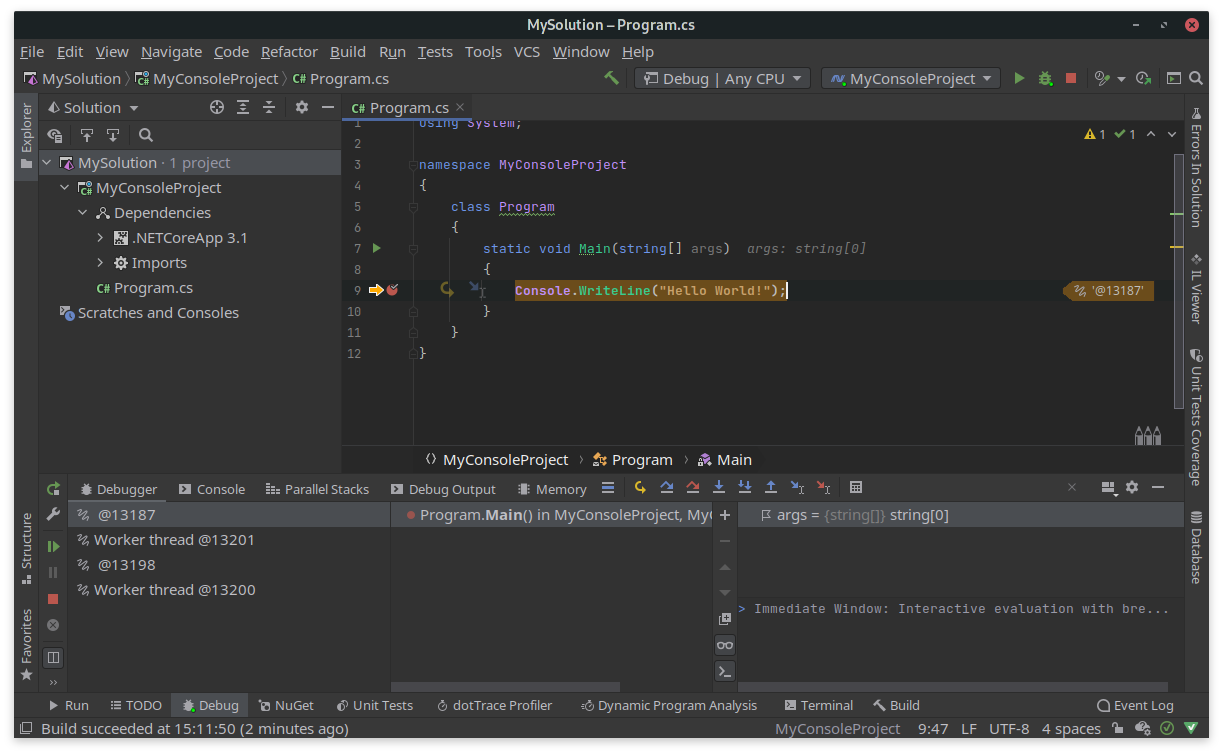
\includegraphics[width=.6\linewidth]{img/rider-6}
        \end{center}
        %
        \begin{itemize}
            \item while suspended, you may \alert{inspect} the current status of a program execution
            %
            \begin{itemize}
                \item[eg] variables values, content of objects, call stacks, etc.
            \end{itemize}
            \item you may also make the program proceed \alert{step-by-step}
        \end{itemize}

    \end{enumerate}

\end{frame}

\section{\csharp Syntax}

\begin{frame}{\csharp Programs}
    A simple \csharp program is a \alert{\texttt{.cs} file}
    %
    \begin{itemize}
        \item containing at least a \alert{namespace} definition
        %
        \begin{itemize}
            \item containing at least a \alert{class} definition
            %
            \begin{itemize}
                \item containing at least a \alert{\texttt{static void Main(\ldots)}} method
            \end{itemize}
        \end{itemize}
    \end{itemize}

    \bigskip

    The program may include other namespaces, classes, interfaces, delegates, or structures definitions
    %
    \begin{itemize}
        \item some of these may in turn include other methods definitions
    \end{itemize}

    \bigskip

    Apart from architectural aspects, the behaviour of \csharp programs is detemined by the \alert{bodies} of methods
    %
    \begin{itemize}
        \item which contain the actual procedural code
    \end{itemize}

    \bigskip

    Procedural aspects of \csharp are really close to the ones of C
    %
    \begin{itemize}
        \item[$\rightarrow$] here we quickly recall the major aspects
    \end{itemize}
\end{frame}

\begin{frame}{A Simple Procedural Program in \csharp}

    The following program considers each command-line argument as a person's name
    %
    \begin{itemize}
        \item it outputs a \alert{\texttt{`Hello PERSON!'}} line for each input argument 
    \end{itemize}

    \lstinputlisting[basicstyle=\tiny\ttfamily]{\codepath{ExampleProject/Program.cs}}


    \begin{itemize}
        \item it exemplifies all procedural aspects of the \csharp syntax
    \end{itemize}

\end{frame}

\begin{frame}[allowframebreaks]{Quick Overview of the \csharp Procedural Syntax}
    \begin{exampleblock}{Notational Conventions}
        \begin{itemize}
            \item \texttt{\cscat{Text within angular brackets}} 
            %
            \begin{itemize}
                \item denote something the developer must write
            \end{itemize}
            \item \texttt{\csopt{Text within square brackets}} 
            %
            \begin{itemize}
                \item denote optional parts
            \end{itemize}
            \item \texttt{\csalt{Text within parentesis | with pipes}} 
            %
            \begin{itemize}
                \item denote alternatives
            \end{itemize}
         \end{itemize}
    \end{exampleblock}

    \framebreak

    \begin{block}{Variable definition \csopt{and assignment}}
        \begin{center}\ttfamily
            \cscat{Type} \cscat{Variable Name}\csopt{ = \cscat{Expression}};
        \end{center}
        %
        \begin{itemize}
            \item \texttt{\cscat{Expression}} must return an instance of \texttt{\cscat{Type}}
            \item if the assignment part is missing, the variable is initialised to the default value of \texttt{\cscat{Type}}
            %
            \begin{itemize}
                \item[ie] 0 for numbers, \texttt{false} for booleans, \texttt{null} for reference types
            \end{itemize}
        \end{itemize}
    \end{block}

    \codeview{3}{9}{14}{\tiny}{\codepath{Snippets/Snippet1Variables.cs}}

    \framebreak

    \begin{block}{Assignment Statement}
        \begin{center}\ttfamily
            \cscat{Selection Expression} = \cscat{Expression};
        \end{center}
        %
        \begin{itemize}
            \item where \texttt{\cscat{Selection Expression}} is commonly something of the form:
            %
            \begin{center}\ttfamily\scriptsize
                \cscat{Other Variable}.\csalt{Property | Field | Method Invocation}.\cscat{Variable}
            \end{center}
            \item and \texttt{\cscat{Variable}} is what is being assigned
            \item and \texttt{\cscat{Expression}} must return an instance of the \texttt{\cscat{Type}} of \cscat{Variable}
        \end{itemize}
    \end{block}

    \codeview{2}{17}{17}{\tiny}{\codepath{Snippets/Snippet1Variables.cs}}

    \codeview{3}{21}{25}{\tiny}{\codepath{Snippets/Snippet1Variables.cs}}

    \framebreak

    \begin{block}{Expressions}
        Any combination of 
        %
        \begin{itemize}
            \item literals (i.e., raw numbers, booleans, or strings),
            \item variables,
            \item method invocations,
            \item constructor invocations,
            \item arrays initialisers,
            \item \csharp operators,
            \item lambda expressions, 
            \item and many others.
        \end{itemize}
    \end{block}

    \begin{alertblock}{Main \csharp Operators \hfill {\tiny (cf. \url{https://docs.microsoft.com/dotnet/csharp/language-reference/operators})}}
        \begin{itemize}
            \item OOP-Related: \op{.}, method call \op{\operand{}(\operand{})}   
            \item Index-Related: indexed access \op{\operand{}[\operand{}]} 
            \item Type Manipulation: \op{as}, \op{typeOf}, \op{is}, cast \op{(\operand{})\operand{}} 
            \item Arithmetic: \op{+}, \op{-}, \op{*}, \op{/}, \op{\%}, \op{++}, \op{--}
            \item Boolean: \op{\&\&}, \op{||}, \op{!}
            \item Bitwise: \op{\&}, \op{|}, \op{\textasciicircum}, \op{~}, \op{<<}, \op{>>} 
            \item Comparison: \op{==}, \op{!=}, \op{<}, \op{>}, \op{>=}, \op{<=}
            \item Null-Related: \op{?.}, \op{??}, \op{\operand{}?[\operand{}]} 
            \item Conditional:  \op{\operand{}?\operand{}:\operand{}}, \op{switch}
            \item Others:  \op{with}, \op{await}, etc.
        \end{itemize}
    \end{alertblock}

    \codeview{3}{9}{17}{\tiny}{\codepath{Snippets/Snippet2Expressions.cs}}

    \framebreak

    \begin{block}{Method Invocation Statement}
        \begin{center}\ttfamily
            \cscat{Selection Expression}(\cscat{Param List});
        \end{center}
        %
        \begin{itemize}
            \item where \texttt{\cscat{Selection Expression}} is commonly something of the form:
            %
            \begin{center}\ttfamily\scriptsize
                \cscat{Other Variable}.\csalt{Property | Field | Method Invocation}.\cscat{Method}
            \end{center}
            \item and \texttt{\cscat{Method}} is what is being invoked
            \item while \texttt{\cscat{Param List}} is a \emph{comma-separated} list of \texttt{\cscat{Expression}}
            %
            \begin{center}\ttfamily\scriptsize
                \cscat{Other Variable}.\csalt{Property | Field | Method Invocation}.\cscat{Variable}
            \end{center}
            \item and the types and the amounts of params is coherent with the ones \cscat{Method} formally declares
        \end{itemize}
    \end{block}

    \codeview{3}{10}{12}{\tiny}{\codepath{Snippets/Snippet3Methods.cs}}

    \framebreak

    \begin{block}{If Construct}
        \begin{center}\ttfamily
            if (\cscat{Expression}) \{ \cscat{Block1} \}
            \csopt{ else \{ Block2 \} }
        \end{center}
        %
        \begin{itemize}
            \item where \texttt{\cscat{Expression}} must return an instance of \texttt{Boolean}
            \item and \texttt{\cscat{Block1}} and \texttt{\cscat{Block2}} are blocks of statements with their own inner scopes
            \item Semantics: \texttt{\cscat{Block1}} is executed if \texttt{\cscat{Expression}} returns \texttt{true}, whereas \texttt{\cscat{Block2}} is executed otherwise
        \end{itemize}
    \end{block}

    \begin{alertblock}{Optional Brackets in If Constructs}
        \begin{itemize}
            \item Brackets may be omitted around \texttt{\cscat{Block1}} or \texttt{\cscat{Block2}} \ldots
            \item \ldots if \emph{and only if} the block contains \alert{just one} statement 
            \item Thus writing
            \begin{center}\ttfamily\footnotesize
                if (\cscat{E1}) \{ \cscat{B1} \} else if (\cscat{E2}) \{ \cscat{B2} \} else \{ \cscat{B3} \}
            \end{center}
            is equal to writing
            \begin{center}\ttfamily\footnotesize
                if (\cscat{E1}) \{ \cscat{B1} \} else \alert{\{} if (\cscat{E2}) \{ \cscat{B2} \} else \{ \cscat{B3} \} \alert{\}}
            \end{center}
        \end{itemize}
    \end{alertblock}

    \codeview{3}{10}{22}{\tiny}{\codepath{Snippets/Snippet4Conditions.cs}}

    \framebreak

    \begin{block}{For-Loop Construct}
        \begin{center}\ttfamily
            for (\csopt{\cscat{Init}}; \csopt{\cscat{Condition}}; \csopt{\cscat{Last}}) \{ \cscat{Block} \}
        \end{center}
        %
        \begin{itemize}
            \item where \cscat{Init} is an optional variable definition statement
            %
            \begin{itemize}
                \item (which defines no variable if missing) 
            \end{itemize}
            \item and \texttt{\cscat{Condition}} is an optional expression returning an instance of \texttt{Boolean}
            %
            \begin{itemize}
                \item (which defaults to \texttt{true} if missing) 
            \end{itemize}
            \item where \cscat{Last} is an optional statement
            %
            \begin{itemize}
                \item (which does nothing if missing) 
            \end{itemize}
            \item Semantics: \texttt{\cscat{Init}} is executed first, then \texttt{\cscat{Block}} is executed 0, 1, or more times, as long as \cscat{Condition} evaluates to \texttt{true}.
            %
            \texttt{\cscat{Condition}} is evalued before each repetition.
            %
            If it evaluates to \texttt{false}, the loop is interrupted.
            %
            After each repetition, and before \texttt{\cscat{Condition}} is evalued again, the \texttt{\cscat{Last}} statement is (re-)executed
        \end{itemize}
    \end{block}

    \codeview{3}{10}{18}{\tiny}{\codepath{Snippets/Snippet5Loops.cs}}

    \lstinputlisting{snippets/for-cycle-result.txt}

    \framebreak

    \begin{block}{While-Do-Loop Construct}
        \begin{center}\ttfamily
            while (\cscat{Condition}) \{ \cscat{Block} \}
        \end{center}
        %
        \begin{itemize}
            \item where \texttt{\cscat{Condition}} is an expression returning an instance of \texttt{Boolean}

            \item Semantics: \texttt{\cscat{Block}} is executed 0, 1, or more times, as long as \cscat{Condition} evaluates to \texttt{true}.
            %
            \texttt{\cscat{Condition}} is always evalued before each repetition, and the repetition is performed only if it evaluates to \texttt{true}, otherwise the loop is interrupted
        \end{itemize}
    \end{block}

    \codeview{3}{23}{34}{\tiny}{\codepath{Snippets/Snippet5Loops.cs}}

    \framebreak

    \begin{block}{Do-While-Loop Construct}
        \begin{center}\ttfamily
            do \{ \cscat{Block} \} while (\cscat{Condition})
        \end{center}
        %
        \begin{itemize}
            \item where \texttt{\cscat{Condition}} is an expression returning an instance of \texttt{Boolean}

            \item Semantics: \texttt{\cscat{Block}} is executed 1, or multiple times, as long as \cscat{Condition} evaluates to \texttt{true}
            %
            \texttt{\cscat{Condition}} is always evalued before each repetition, and the repetition is performed only if it evaluates to \texttt{true}, otherwise the loop is interrupted
        \end{itemize}
    \end{block}

    \codeview{3}{39}{50}{\tiny}{\codepath{Snippets/Snippet5Loops.cs}}

    \framebreak

    \begin{block}{Method Definition Construct}
        \begin{center}\ttfamily
            \cscat{Type} \cscat{Method Name} ( \cscat{Type1} \cscat{Arg1}, \ldots, \cscat{TypeN} \cscat{ArgN} )
            \\ 
            \{ Block \}
        \end{center}
        %
        \begin{itemize}
            \item where \texttt{\cscat{Type}} is the \alert{return type} of the method
            \item and each \texttt{\cscat{Type$_i$} \cscat{Arg$_i$}} is a \alert{formal} argument 
            %
            \begin{itemize}
                \item whose name is \texttt{\cscat{Arg$_i$}} and whose type is \texttt{\cscat{Type$_i$}}
            \end{itemize}
            \item and all computational paths within \texttt{\cscat{Block}} end with a statement of the form, unless \texttt{\cscat{Type} $=$ \alert{void}}
            \begin{center}\ttfamily
                return \cscat{Expression}
            \end{center}
            where \texttt{\cscat{Expression}} evaluates to an instance of \texttt{\cscat{Type}}
        \end{itemize}
    \end{block}

    \codeview{2}{15}{32}{\tiny}{\codepath{Snippets/Snippet3Methods.cs}}
\end{frame}

\section{\dotnet Type System}

\subsection{Reference Types vs. Value Types}

\begin{frame}{\dotnet Type System -- Overview}
    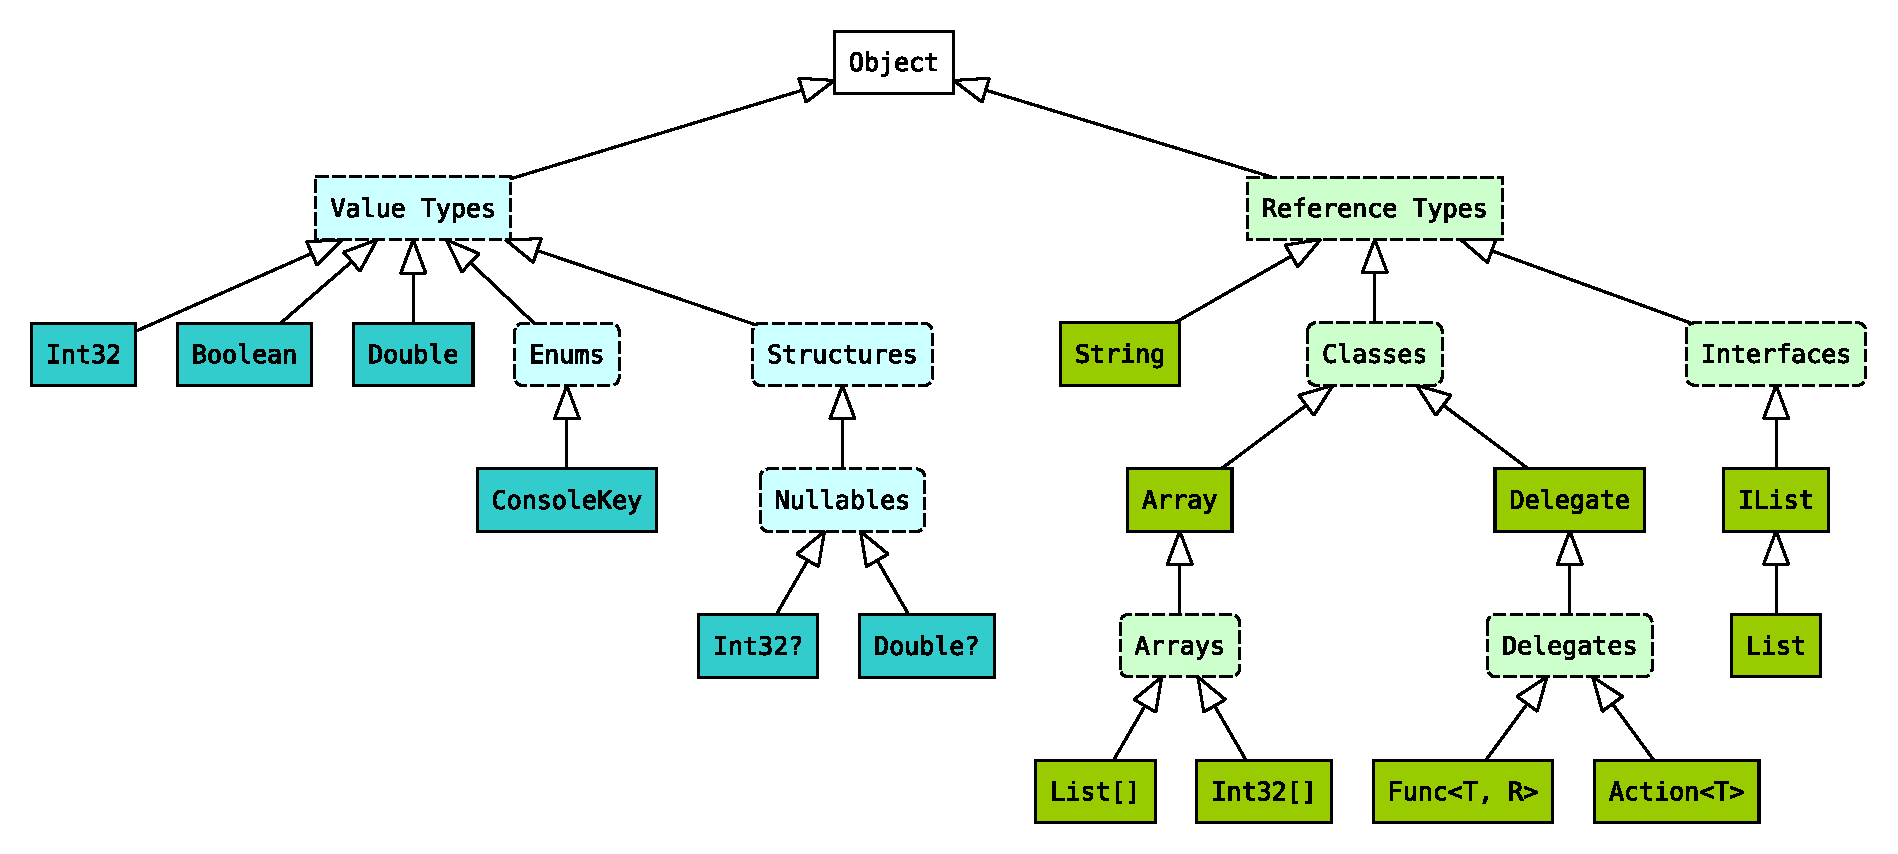
\includegraphics[width=\linewidth]{img/type-system.pdf}

    \begin{block}{Type System Insight}
        \begin{itemize}
            \item Type $\approx$ set of admissible values (for variables)
            \item \texttt{A} sub-type of \texttt{B} $\implies$ \texttt{B} $\subset$ \texttt{A}
        \end{itemize}
    \end{block}
\end{frame}

\begin{frame}{\dotnet Type System -- General Principles}
    \begin{itemize}
        \item \texttt{Object} is the supertype of all types
        %
        \begin{itemize}
            \item[$\rightarrow$] every object is an instance of \texttt{Object}
        \end{itemize}

        \vfill

        \item There are two main categories of types: % \alert{Value} and \alert{Reference} Types
        %
        \begin{description}\small
            \item[Value Types:] are passed \alert{by type} (i.e. \emph{cloned}) among method calls
            \item[Reference Types:] are passed \alert{by reference} (i.e. \emph{shared}) among method calls 
        \end{description}

        \vfill

        \item The symbol \alert{\texttt{null}} represents the lack of reference
        %
        \begin{itemize}
            \item it is an admissible value for \alert{all} reference types
            \item it is \alert{not} admissible value for \alert{any} value type
        \end{itemize}

        \vfill

        \item All enums, nullables, and \alert{custom structures} are \emph{value types}       
        
        \vfill

        \item All arrays, delegates, and \alert{custom classes/interfaces} are \emph{reference types}
        
        \vfill

        \item Bult-in types such as \texttt{Boolean}, \texttt{Int32}, \texttt{Double}, etc. are \emph{value types}  
        %
        \begin{itemize}
            \item their default value is \texttt{false} (for \texttt{Boolean}s) and \texttt{0} (for numbers)
        \end{itemize}
        
        \vfill

        \item Bult-in types such as \texttt{String}, \texttt{Array}, \texttt{List}, etc. are \emph{reference types}
        %
        \begin{itemize}
            \item their default value is \texttt{null}
        \end{itemize}

    \end{itemize}
\end{frame}

\subsubsection{Built-in Types}

\begin{frame}{\dotnet Built-in Types}\centering
    \begin{table}[]
        \resizebox{\textwidth}{!}{
        \begin{tabular}{c|c|c|c|c}
            \textbf{Name}    & \textbf{Keyword} & \textbf{Category} & \textbf{Size} & \textbf{Description}  \\
            \hline\hline
            \texttt{Boolean} & \texttt{bool}    & \emph{val} & 1             & either \texttt{true} or \texttt{false} \\
            \texttt{Char}    & \texttt{char}    & \emph{val} & 2             & UTF-16 characters \texttt{`U+0000'} \ldots \texttt{`U+FFFF'} \\
            \texttt{Byte}    & \texttt{byte}    & \emph{val} & 1             & integers in $0 \ldots (2^{8}-1)$ \\
            \texttt{SByte}   & \texttt{sbyte}   & \emph{val} & 1             & integers in $-2^{7} \ldots (2^{7}-1)$ \\
            \texttt{Int16}   & \texttt{short}   & \emph{val} & 2             & integers in $-2^{15} \ldots (2^{15}-1)$ \\
            \texttt{UInt16}  & \texttt{ushort}  & \emph{val} & 2             & integers in $0 \ldots (2^{16}-1)$ \\
            \texttt{Int32}   & \texttt{int}     & \emph{val} & 4             & integers in $-2^{31} \ldots (2^{31}-1)$ \\
            \texttt{UInt32}  & \texttt{uint}    & \emph{val} & 4             & integers in $0 \ldots (2^{32}-1)$ \\
            \texttt{Int64}   & \texttt{long}    & \emph{val} & 8             & integers in $-2^{63} \ldots (2^{63}-1)$ \\
            \texttt{UInt64}  & \texttt{ulong}   & \emph{val} & 8             & integers in $0 \ldots (2^{64}-1)$ \\
            \texttt{Float}   & \texttt{float}   & \emph{val} & 4             & abs in $1.5\times 10^{-45} \ldots 3.4\times 10^{38}$ \\
            \texttt{Double}  & \texttt{double}  & \emph{val} & 8             & abs in $5.0\times 10^{-324} \ldots 1.7\times 10^{308}$ \\
            \texttt{Decimal} & \texttt{decimal} & \emph{val} & 16            & abs in $1.0\times 10^{-28} \ldots 7.9228 \times 10^{28}$ \\
            \hdashline
            \texttt{Object}  & \texttt{object}  & \emph{ref} & O(1)          & anything \\
            \texttt{String}  & \texttt{string}  & \emph{ref} & O($n$)   & sequences of $n$ UTF-16 characters \\
        \end{tabular}
        }
    \end{table}

    \tiny
    (cf. \url{https://docs.microsoft.com/dotnet/csharp/language-reference/builtin-types/built-in-types})

\end{frame}

\begin{frame}[allowframebreaks]{Built-in Types Instantiation}
    \begin{block}{Literals}\centering
        Literal $\approx$ \dotnet code representing an instance of some built-in type
    \end{block}

    \begin{exampleblock}{Alphanumeric Literals}
        \begin{description}
            \item[characters:] single-quoted character or escape sequence
            %
            \begin{itemize}
                \item[eg] \literal{'a'}, \literal{'B'}, \literal{'\bs{}n'}, \literal{'\bs{}uABCD'}, etc.
            \end{itemize} 
             
            \item[strings:] double-quoted sequence of characters or escape sequences
            %
            \begin{itemize}
                \item[eg] \literal{"Hello World"}, \literal{"Hello\bs{}nWorld"}, etc.
            \end{itemize} 

            \item[literal strings:] double-quoted sequence of characters prefixed by \literal{@}
            %
            \begin{itemize}
                \item[eg] \literal{@"Hello World"}, \literal{@"Hello\bs{}nWorld"}, etc.
            \end{itemize} 
            
            \item[string interpolation:] double-quoted sequence of characters or escape sequences prefixed by \literal{\$} and possibly containing expressions within braces
            %
            \begin{itemize}
                \item[eg] \literal{\$"Age: \{person.Age\} yo"}, \literal{\$"1+1 = \{3-1\}"}, etc.
            \end{itemize}  
        \end{description}
    \end{exampleblock}

    \begin{alertblock}{Beware of Escape Sequences!}
        \begin{itemize}
            \item[ie] sequences of characters aimed at representing a single particular character
            \item cf. \url{https://csharpindepth.com/articles/Strings} 
            \item use literal strings if you want escape sequences to be ignored!
        \end{itemize}
    \end{alertblock}

    \begin{exampleblock}{Numeric Literals}
        \begin{description}
            \item[booleans:] there are just 2 literals: \literal{true} and \literal{false}
            
            \item[integers:] integer numbers with optional sign (\literal{0}, \literal{-1}, \literal{1}, \literal{+1}, etc.)

            \item[hexadecimals:] hex numbers with optional sign, prefixed by \literal{0x}/\literal{0X}
            %
            \begin{itemize}
                \item[eg] \literal{0x0}, \literal{0x1A}, \literal{-0Xff}, etc.
            \end{itemize} 

            \item[long integers]: integer literals suffixed by \literal{L} or \literal{l} (prefer \texttt{L})
            %
            \begin{itemize}
                \item[eg] \literal{0L}, \literal{-1L}, \literal{+0xFFL}, etc.
            \end{itemize}  

            \item[unsigned integers]: integer literals suffixed by \literal{u} or \literal{U} and no sign
            
            \item[doubles:] any dotted number, optionally signed, or suffixed by either an exponent or by \literal{D}/\literal{d} (prefer \texttt{d})
            %
            \begin{itemize}
                \item[eg] \literal{0.0}, \literal{1.2}, \literal{-3.4}, \literal{5d}, \literal{.6}, \literal{-1.2e3}, \literal{+4.5e-6}
            \end{itemize}   
            
            \item[floats:] same as above, but ending with \literal{F}/\literal{f}
            
            \item[decimals:] same as above, but ending with \literal{M}/\literal{m}
        \end{description}
    \end{exampleblock}

    \begin{exampleblock}{Parsing Numbers (i.e. Instantiating Numbers out of Strings)}
        \begin{itemize}
            \item All built-in numeric types come with a \alert{static factory method} for parsing, named \texttt{Parse}
            %
            \begin{itemize}
                \item[eg] \texttt{int.Parse("-321")} or \texttt{Int32.Parse("+123")}
                \item[eg] \texttt{bool.Parse("false")} or \texttt{Boolean.Parse("true")}
                \item[eg] \texttt{ulong.Parse("54321")} or \texttt{UInt64.Parse("12345")} 
                \item[eg] \texttt{double.Parse("5.4")} or \texttt{Double.Parse("4.5")}  
            \end{itemize}
        \end{itemize}
    \end{exampleblock}

    \begin{block}{Manipulating Built-in Types via Operators}
        \begin{itemize}
            \item Built-in types are \alert{immutable}
            \item So, combining their instances via operators creates novel instances 
            \item Racall that the \texttt{+} operator means ``concatenation'' to strings
        \end{itemize}
    \end{block}
\end{frame}

\subsubsection{Custom Types}

\begin{frame}{Custom \dotnet Types}
    \begin{exampleblock}{Custom Reference Types}\centering
        May be created by defining \alert{\texttt{class}es}, \alert{interfaces}, or \alert{delegates}
        %
        \begin{itemize}
            \item we will soon delve into the details of how to do so
        \end{itemize}
    \end{exampleblock}

    \begin{exampleblock}{Custom Value Types}\centering
        May be created by defining \alert{\texttt{struct}ures} or \alert{\texttt{enum}s}
        %
        \begin{itemize}
            \item this is an advanced aspect we will eventually present
        \end{itemize}
    \end{exampleblock}

\end{frame}

\begin{frame}{Custom Types Instantiation}
    \begin{block}{Constructors}
        \begin{itemize}
            \item Both custom classes and structores are instantiated via \alert{constructors}
            %
            \begin{itemize}
                \item provided that these are \alert{visible}
            \end{itemize}

            \item In some cases, \alert{static factory methods} may be preferred
            %
            \begin{itemize}
                \item this is an advanced programming pattern that we will eventually explain
                \item yet, some \dotnet class may rely on this pattern
            \end{itemize}
        \end{itemize}
    \end{block}
\end{frame}

\subsubsection{Arrays}

\begin{frame}[allowframebreaks]{\dotnet Arrays}
    \begin{block}{$N$-dimensional arrays (a.k.a. matrices) definition}
        Let \texttt{\textit{T}} by a \dotnet type of any sort, then 
        %
        \begin{description}
            \item[\texttt{\textit{T}\alert{[]}}] denotes the \alert{array of \texttt{\textit{T}}} type
            \item[\texttt{\textit{T}\alert{[,]}}] denotes the \alert{2-dimensional array of \texttt{\textit{T}}} type 
            \item[\texttt{\textit{T}\alert{[,,]}}] denotes the \alert{3-dimensional array of \texttt{\textit{T}}} type 
            \item[\ldots]
        \end{description}

        A $N$-dimensional array of \texttt{\textit{T}} is an \alert{ordered} data structure contaning $D_1 \times \ldots \times D_N$ instances of \texttt{\textit{T}}
    \end{block}

    {\tiny (cf. \url{https://docs.microsoft.com/dotnet/csharp/programming-guide/arrays/})}

    \begin{alertblock}{Jagged arrays}
        The definition of arrays can be applied to array types as well:
        %
        \begin{description}
            \item[\texttt{\textit{T}\alert{[][]}}] denotes the \alert{array of \emph{arrays of} \texttt{\textit{T}}} type
            \item[\texttt{\textit{T}\alert{[][][]}}] denotes the \alert{array of \emph{arrays of arrays of} \texttt{\textit{T}}} type
            \item[\texttt{\textit{T}\alert{[][,]}}] denotes the \alert{array of \emph{2-dimensional arrays of} \texttt{\textit{T}}} type
            \item[\texttt{\textit{T}\alert{[,,][]}}] denotes the \alert{3-dimensional array of \emph{arrays of} \texttt{\textit{T}}} type
        \end{description}

        (Left $\rightarrow$ outer, right $\rightarrow$ inner)
    \end{alertblock}

    \begin{exampleblock}{Arrays features}
        \begin{itemize}
            \item All array types are \alert{reference} types
            %
            \begin{itemize}
                \item arrays of value types are reference types as well
            \end{itemize}

            \item All array types are subtypes of the \texttt{Array} class

            \item Arrays are constructed by sizes, i.e. $D_1, \ldots, D_N$ are user-provided
            %
            \begin{itemize}
                \item so memory can be contigously allocated
                \item items are initialised to their default values
            \end{itemize}

            \item All array types come with 3 useful properties/methods:
            %
            \begin{description}
                \item[\texttt{Rank}] returning the total amount of dimensions of the array (i.e. $N$)
                \item[\texttt{Length}] returning the total amount of items in the array (i.e. $D_1 \times \ldots \times D_N$)
                \item[\texttt{GetLength($i$)}] returning the total amount of items along the $i$-th dimension (i.e. $D_i$)
            \end{description}

            \item Access to items is performed via the indexed-access operator:
            %
            \begin{center}
                \op{\operand[array][\operand[index$_1$, \ldots, index$_N$]]}  
            \end{center}
        \end{itemize}
    \end{exampleblock}
\end{frame} 

\begin{frame}[allowframebreaks]{Array Types Instantiation}
    \begin{block}{About Arrays Instantiation}
        Arrays instantiation may be performed in two ways:
        %
        \begin{itemize}
            \item array \alert{constructors}, which instantiate an array by size(s)
            %
            \begin{itemize}
                \item they have a slightly different syntax than ordinary objects constructors
            \end{itemize}

            \item literal array expressions
        \end{itemize}
        %
        or via a combination of the two.
    \end{block}

    \begin{exampleblock}{Constructors for $N$-dimensional Arrays of \texttt{\textit{T}}}
        \begin{center}\ttfamily
            \textit{T}[\alert{,,}\ldots{}] \cscat{Var Name} = \alert{new} \textit{T}[\alert{$D_1$}, \alert{$D_2$}, \ldots];
        \end{center}
        %
        \begin{itemize}
            \item Number of commas in the left-hand side: $N-1$
            \item Number of sizes in the right-hand side: $N$
        \end{itemize}
    \end{exampleblock}

    \begin{exampleblock}{Literal Array Expressions for $N$-dimensional Arrays of \texttt{\textit{T}}}
        \begin{center}\ttfamily
            \textit{T}[\alert{,,}\ldots{}] \cscat{Var Name} = \alert{new} \textit{T}[\alert{,,}\ldots{}] 
                \alert{\{\ldots\{} \cscat{Item$_1$}, \cscat{Item$_2$}, \ldots  \alert{\}\ldots\}};
        \end{center}
        %
        \begin{itemize}
            \item Number of commas in the left-hand side: $N-1$
            \item Number of nesting levels of braces in the right-hand side: $N$
            \item Repeating \texttt{\textit{T}[\alert{,,}\ldots{}]} may be avoided in the right-hand side
        \end{itemize}
    \end{exampleblock}

    \framebreak
    
    \codeview{3}{9}{24}{\tiny}{\codepath{Snippets/Snippet6Arrays.cs}}

\end{frame}

\begin{frame}[allowframebreaks]{Accessing Arrays Items}
    \begin{block}{Notable Aspects of Arrays}
        \begin{itemize}
            \item Arrays are \alert{mutable} data types
            \item So they can be accessed both for \alert{reading or changing} their items
            \item Array sizes \alert{cannot} be altered
            %
            \begin{itemize}
                \item unless \alert{a copy} of the whole array is performed
            \end{itemize}
        \end{itemize}
    \end{block}

    \begin{exampleblock}{Reading an Item from a $N$-dimensional Array \texttt{\textit{T}}}
        \begin{center}\ttfamily
            \cscat{Array Variable}\alert{[}\cscat{Index$_1$}, \ldots, \cscat{Index$_N$}\alert{]}
        \end{center}
        %
        \begin{itemize}
            \item where each \texttt{\cscat{Index$_i$}} is an integer-returning expression
            \item and the whole expression returns an instance of \texttt{\textit{T}}
        \end{itemize}
    \end{exampleblock}

    \begin{exampleblock}{Changing an Item in a $N$-dimensional Array \texttt{\textit{T}}}
        \begin{center}\ttfamily
            \cscat{Array Variable}\alert{[}\cscat{Index$_1$}, \ldots, \cscat{Index$_N$}\alert{]} \alert{= \cscat{Value}}
        \end{center}
        %
        \begin{itemize}
            \item where each \texttt{\cscat{Index$_i$}} is an integer-returning expression
            \item and \texttt{\cscat{Value}} is an expression returning an instance of \texttt{\textit{T}}
        \end{itemize}
    \end{exampleblock}

    \framebreak

    \codeview{2}{27}{41}{\tiny}{\codepath{Snippets/Snippet6Arrays.cs}}

    \codeview{2}{43}{52}{\tiny}{\codepath{Snippets/Snippet6Arrays.cs}}

\end{frame}

\subsubsection{Nullables}

\begin{frame}[allowframebreaks]{\dotnet Nullables}
    \begin{block}{Nullable types definition}
        Let \texttt{\textit{T}} by a \alert{value} type of any sort, then 
        %
        \begin{description}
            \item[\texttt{\textit{T}\alert{?}}] denotes the \alert{nullable \texttt{\textit{T}}} type
        \end{description}

        A nullable type \texttt{\textit{T}?} can be defined as \texttt{\textit{T}} $\cup$ \{ \texttt{null} \}.
        %
        A variable of type \texttt{\textit{T}?} can be assigned with any admissible value of \texttt{\textit{T}}, \alert{or} with \texttt{null}
        %
        \begin{itemize}
            \item there, \texttt{null} represents an unknown value
        \end{itemize}

        {\tiny (cf. \url{https://docs.microsoft.com/dotnet/csharp/language-reference/builtin-types/nullable-value-types})}
    \end{block}

    \begin{exampleblock}{Nullables features}
        \begin{itemize}
            \item All nullable types are \alert{value} types
            %
            \begin{itemize}
                \item only case of value type having \texttt{null} among its admissible values
            \end{itemize}

            \item The notation \texttt{\textit{T}?} is another way of writing \texttt{Nullable<\textit{T}>}
            %
            \begin{itemize}
                \item which is a \emph{generic} structure
                %
                \begin{itemize}
                    \item[ie] an advanced aspect we will explain later in this course
                \end{itemize}
            \end{itemize}

            \item All nullable types come with some useful properties:
            %
            \begin{description}
                \item[\texttt{HasValue}] returning null if the object is null
                \item[\texttt{Value}] returning the non-null value, if present
            \end{description}

            \item When non-null, nullable-type variables behave like they non-nullable counterparts
            
            \item Intricacies may arise when comibining null and non-null variables in some expression
        \end{itemize}
    \end{exampleblock}
    
\end{frame}

\begin{frame}{Nullable Types Instantiation}
    \begin{block}{}
        \begin{itemize}
            \item Nullable types are instantiated via literals, constructors, or static factory methods
            %
            \begin{itemize}
                \item exactly as their non-nullable counterparts
            \end{itemize}

            \item Except that they can be initialised to \alert{\texttt{null}} as well
        \end{itemize}
    \end{block}

    \codeview{3}{9}{13}{\tiny}{\codepath{Snippets/Snippet7Nullables.cs}}
\end{frame}

\section{Coding Conventions}

\begin{frame}[allowframebreaks]{About Coding Style Conventions}
    \begin{block}{Definition}
        \begin{itemize}
            \item Stylistic rules about how to write good-quality code
            %
            \begin{itemize}
                \item[eg] fields/properties/methods/types names, usage of white spaces, empty lines, comments, etc.
            \end{itemize}

            \item Usually \alert{followed} by all developers in a given community / project
            
            \item Possibily \alert{enforced} by \emph{automatic} tools
            
            \item Aimed at easing:
            %
            \begin{itemize}
                \item interoperability among developers,
                \item readability of the source code, and
                \item the maintainability of the code base
            \end{itemize}
        \end{itemize}
    \end{block}

    \begin{alertblock}{Coding Style Conventions are \textbf{Important}}
        \begin{itemize}
            \item Sticking to some \alert{shared} coding style is \emph{fundamental}
            %
            \begin{itemize}
                \item  especially, when working in \alert{teams}
            \end{itemize}
            
            \item Even if you are working alone, people may eventually join the project, forming a team
            %
            \begin{itemize}
                \item[$\rightarrow$] always act like you are in a team, even when coding alone
            \end{itemize}

            \item Coding conventions are \alert{not} a matter of \alert{taste}
            %
            \begin{itemize}
                \item \alert{do not ignore} some convention just because it appears \alert{ugly} to you
                \item conventions are never ugly/beautiful, nor right/wrong
                \item conventions are important as they are \alert{shared}
            \end{itemize} 

            \item One everybody gets used to conventions, they easy developers' understanding of the code
            %
            \begin{itemize}
                \item[eg] naming conventions help understanding what a symbol is without need to see its definition
                \item[$\rightarrow$] violating a convention is harmful: it misleads code readers  
            \end{itemize}
        \end{itemize}
    \end{alertblock}

    \begin{exampleblock}{\csharp Coding Conventions}\centering
        We stick to the conventions enumerated here:
        \\
        {\tiny \url{https://github.com/dotnet/runtime/blob/main/docs/coding-guidelines/coding-style.md}}
    \end{exampleblock}
    %
    \begin{itemize}
        \item[$\rightarrow$] we provide an overview of most relevant conventions in the next slides 
    \end{itemize}
\end{frame}

\begin{frame}[allowframebreaks]{\csharp Coding Style}

    \begin{block}{Concatenated Words Styles around the World}
        \begin{description}
            \item[\texttt{camelCase}] | \url{https://en.wikipedia.org/wiki/Camel_case}
            \item[\texttt{PascalCase}] | like \texttt{camelCase} but the first letter is uppercase
            \item[\texttt{snake\_case}] |  \url{https://en.wikipedia.org/wiki/Snake_case}
            \item[\texttt{kebab-case}] |  \url{https://it.wikipedia.org/wiki/Kebab_case} 
        \end{description}
        %
        \begin{itemize}
            \item[!] \dotnet conventions mostly rely on \texttt{camelCase} and \texttt{PascalCase}
        \end{itemize}
    \end{block}

    \begin{exampleblock}{Suggested Naming Conventions for \csharp}
        \begin{description}
            \item[\textbf{namespaces} names] are in \texttt{PascalCase} 

            \item[\textbf{type} names] (classes, interfaces, structures, delegates) are in \texttt{PascalCase}  
            %
            \begin{itemize}
                \item[eg] \texttt{String}, \texttt{List}, \texttt{Int32}, \texttt{Action} etc.
            \end{itemize} 

            \item[\textbf{inteface} names] start with a \texttt{`I'} and are in \texttt{PascalCase} 
            %
            \begin{itemize}
                \item[eg] \texttt{IList}, \texttt{ISet}, \texttt{IDictionary} etc.
            \end{itemize} 

            \item[\textbf{abstract class} names] start with \texttt{`Abstract'} and are in \texttt{PascalCase} 
            
            \item[\textbf{field} names] start with a \texttt{`\_'} and are in \texttt{camelCase} 
            
            \item[\textbf{method} names] are in \texttt{PascalCase} 
            
            \item[\textbf{property} names] are in \texttt{PascalCase} 
            
            \item[\textbf{local variables} and \textbf{methods parameters} names] are in \texttt{camelCase} 
            
        \end{description}
        %
        \begin{itemize}
            \item[!] all names are \alert{in English}
        \end{itemize}
    \end{exampleblock}

    \framebreak

    \begin{exampleblock}{Suggested Bracing Conventions for \csharp}
        \csharp bracing style is \alert{Allman's} one\footnote{\tiny(cf. \url{https://en.wikipedia.org/wiki/Indentation_style\#Allman_style})}
        %
        \begin{itemize}
            \item braces are always mandatory, except in \alert{\texttt{else if}} 
            \item open and closed braces always lay their own line
            \item indentation levels of open/closed braces is the same of the clause they belong to
            \item statements within braces are subject to 4-spaces indentation
            \item[!] this style is different from Java's and JavaScript's ones
        \end{itemize}
    \end{exampleblock}

    \begin{exampleblock}{Suggested White Space Conventions for \csharp}
        \begin{itemize}
            \item Indentation exploits 4 spaces \alert{instead of} tabulations
            %
            \begin{itemize}
                \item you may need to enable white characters visualization to spot the difference
            \end{itemize} 
            \item A space is mandatory \alert{before and after} each \alert{infix} operator
            %
            \begin{itemize}
                \item[ie] arithmetic, boolean, bitwise, comparison operators, etc.
                \item[eg] \texttt{`a + b'} is ok, \texttt{`a!=b'} is not ok
            \end{itemize}
            \item Commas require \alert{no space before} and a \alert{single space after}
            %
            \begin{itemize}
                \item[eg] \texttt{`a, b'} is ok, \texttt{`a , b'} or \texttt{`a,b'} are not ok
            \end{itemize} 
            \item Semicolons require \alert{no space before} 
            \item Constructs require \alert{a single space} within name and round parenthesis opening
            %
            \begin{itemize}
                \item[eg] \texttt{`if (\ldots'}, \texttt{`while (\ldots'} or \texttt{`for (\ldots'} are ok
            \end{itemize} 
        \end{itemize}
    \end{exampleblock}

    \begin{exampleblock}{Other Suggested Conventions for \csharp}
        \begin{itemize}
            \item Define variables with \alert{\texttt{var}} only if the type is \alert{obvious and evindent} in that context
            \item Use keywords instead of full names for built-in types
            \item Define \alert{\texttt{readonly}} variables/fields/properties whenever possible
            \item Always specify visibility modifiers explicitly
            \item Prefer conciseness when possible
            \item Order classes members as follows (top-down):
            %
            \begin{enumerate}
                \item fields
                \item constructors
                \item properties (public first)
                \item methods (public first)
                \item static members
            \end{enumerate}
        \end{itemize}
    \end{exampleblock}

    \begin{exampleblock}{Suggested File/Directory Organization for \dotnet}
        \begin{itemize}
            \item One type definition (class, struct, enum, delegate, \ldots) per file
            %
            \begin{itemize}
                \item so that developers may easily locate definitions
            \end{itemize}
            \item Name the file after the type definition it carries
            %
            \begin{itemize}
                \item[eg] \texttt{class Person} defined into \texttt{Person.cs} (or \texttt{Person.vb})
            \end{itemize}
            \item Each project exposes a \alert{root namespace} named after it
            %
            \begin{itemize}
                \item[eg] the root namespace of project \texttt{P} is named \texttt{P}
            \end{itemize}
            \item All source files from a project root directory contain type definitions laying within that project root namespace
            %
            \begin{itemize}
                \item[eg] the file \texttt{P/Person.cs} defines class \texttt{Person} within namespace \texttt{P}
            \end{itemize}
            \item Sub-directories reflect sub-namespaces
            %
            \begin{itemize}
                \item[eg] the file \texttt{P/People/Person.cs} defines class \texttt{Person} within namespace \texttt{P.People}
            \end{itemize}
        \end{itemize}
    \end{exampleblock}

\end{frame}

\begin{frame}{\csharp Coding Style -- Can you spot all the problems?}\centering

    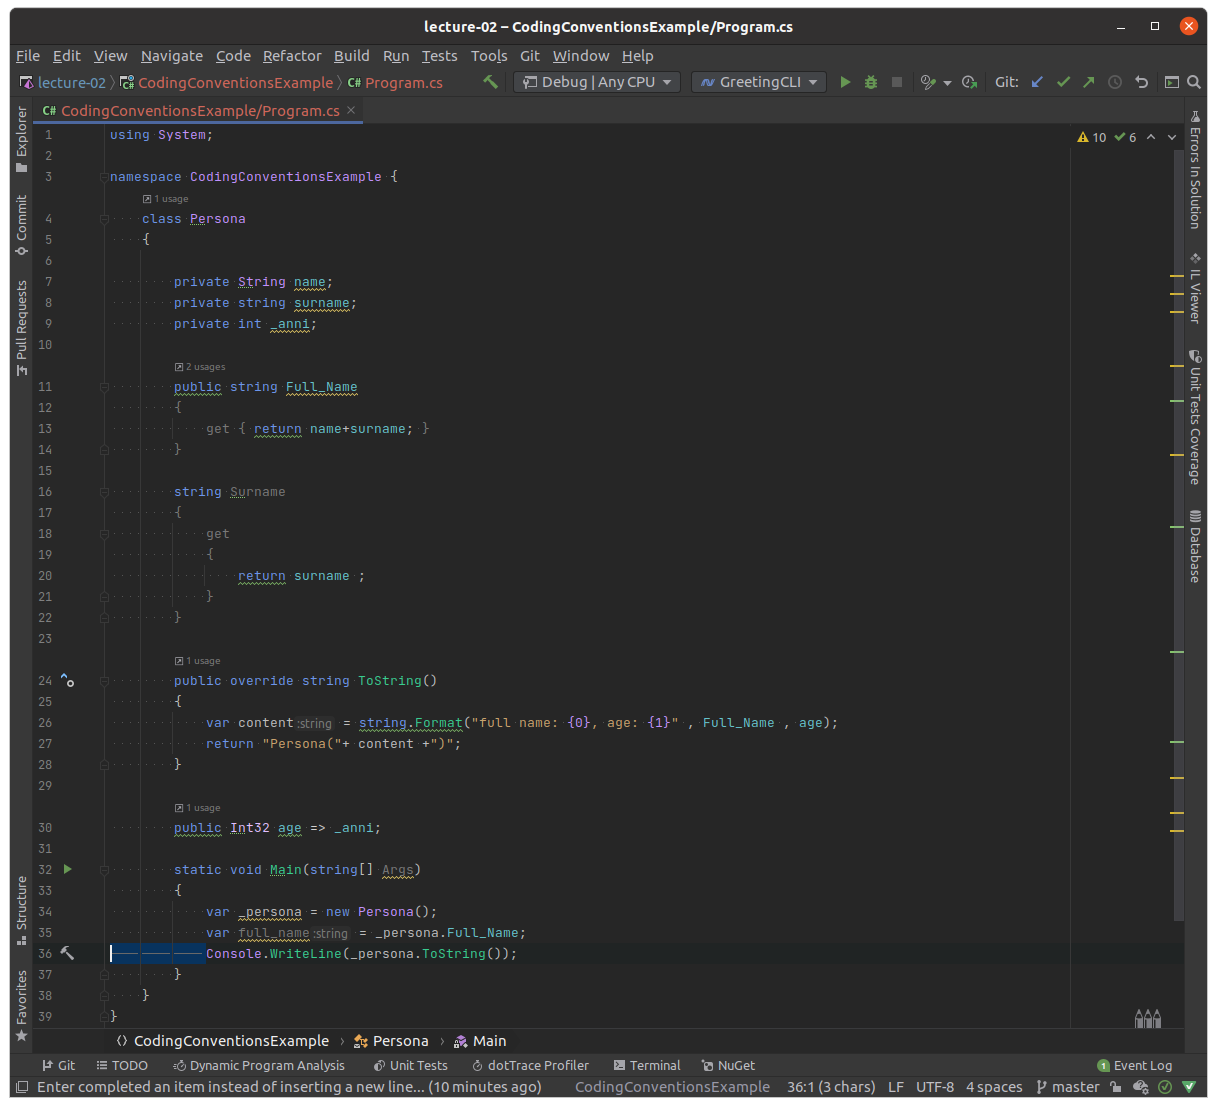
\includegraphics[width=0.7\linewidth]{img/wrong-conventions.png}

\end{frame}

\begin{frame}{\csharp Coding Style -- Can you name all the problems? }\centering

    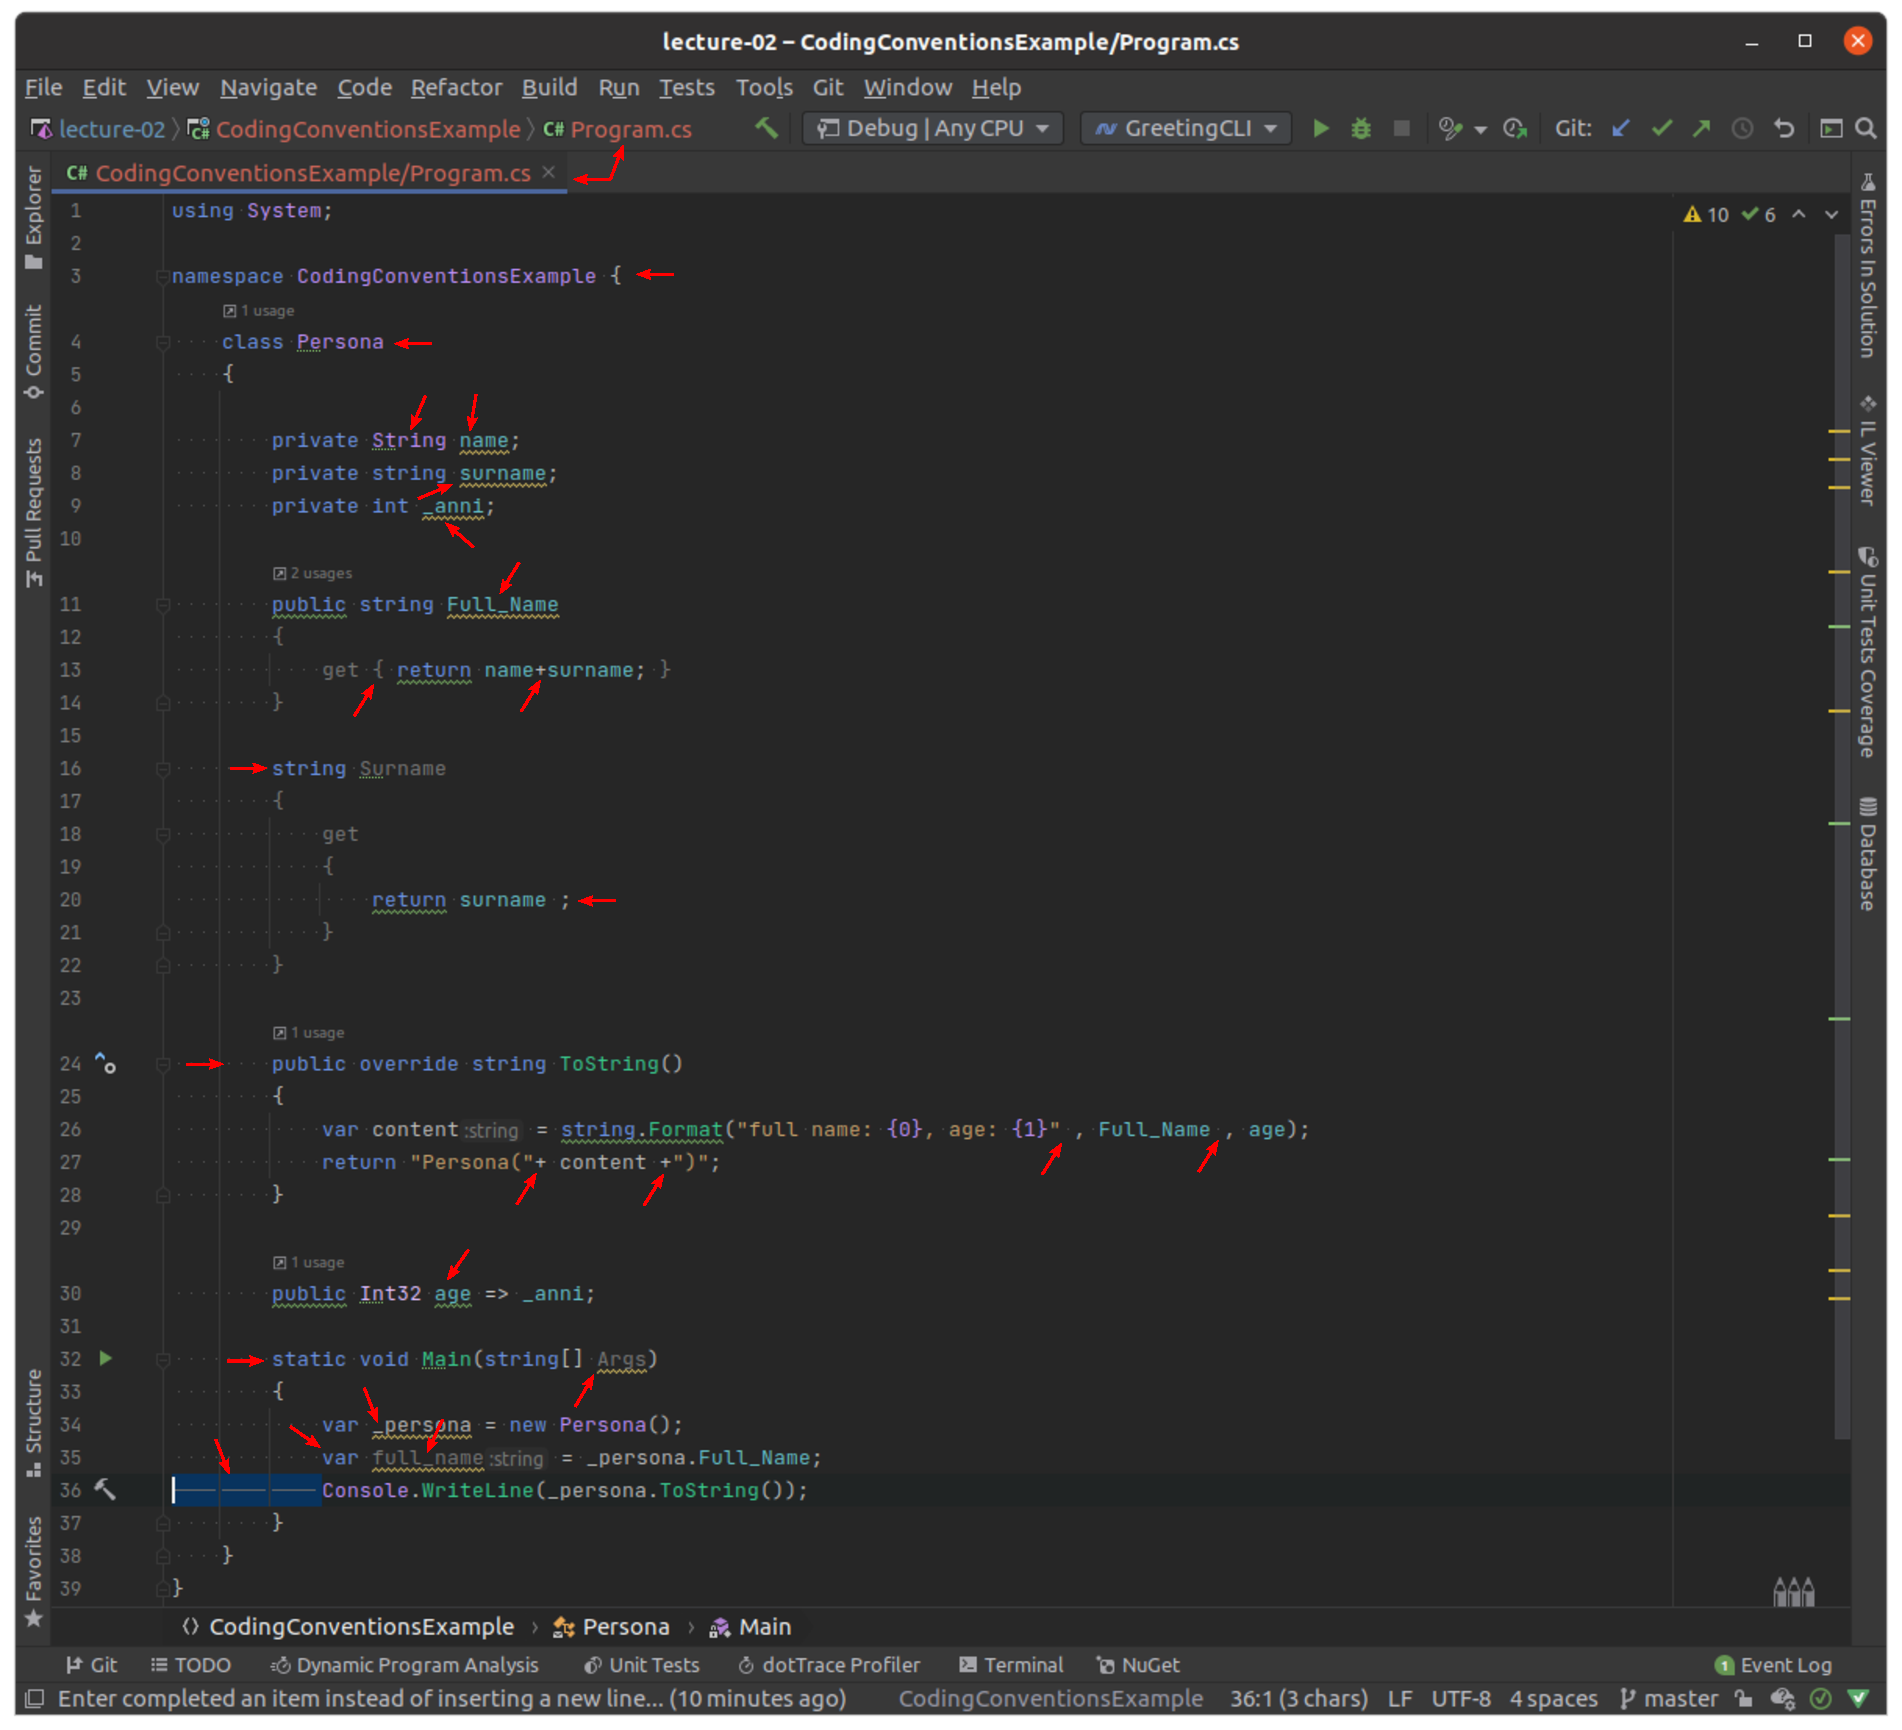
\includegraphics[width=0.7\linewidth]{img/wrong-conventions.pdf}

\end{frame}

\begin{frame}{\csharp Coding Style -- Correct Version }\centering

    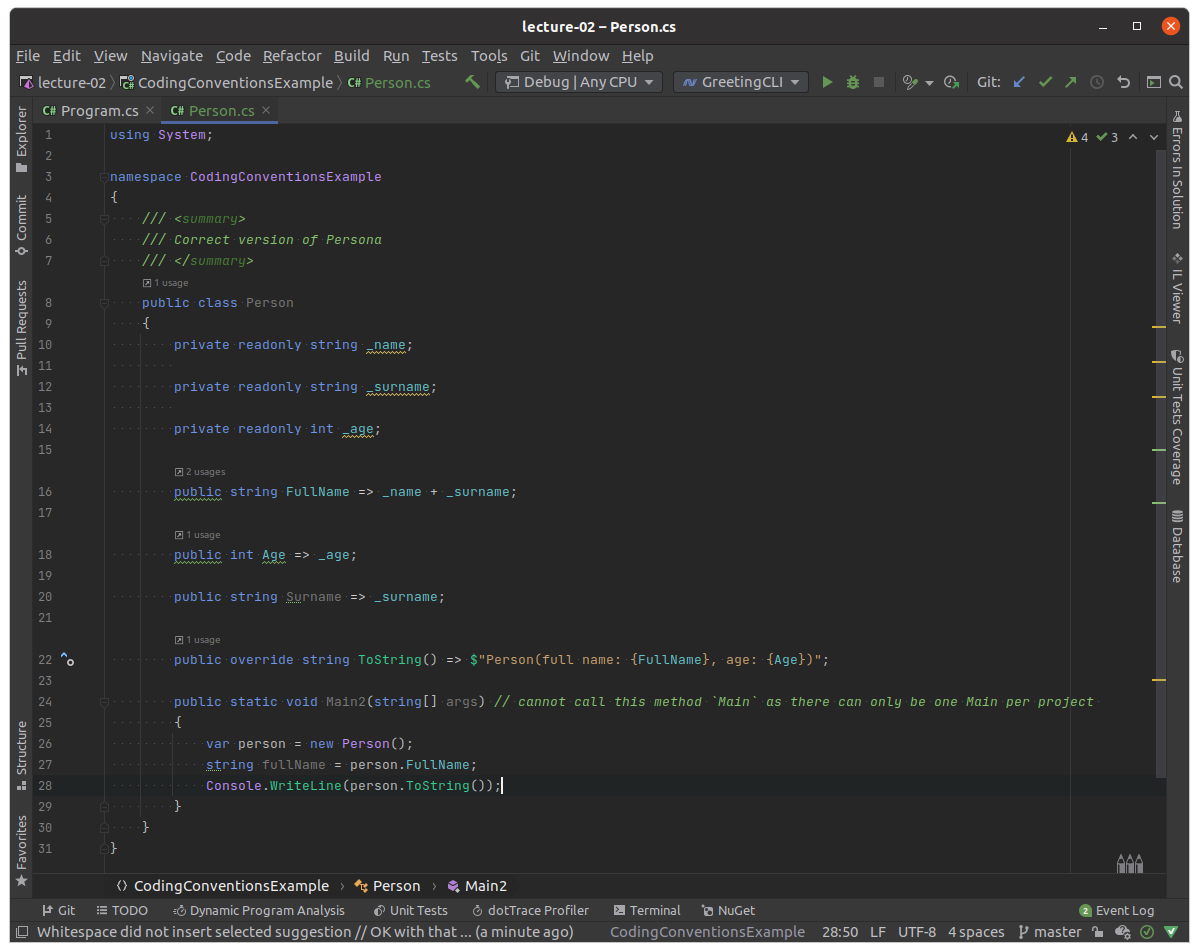
\includegraphics[width=0.8\linewidth]{img/good-conventions.png}

\end{frame}

\end{document}
